% !Mode:: "TeX:UTF-8"
% !TEX encoding = UTF-8 Unicode

%----------------------------------------------------------------------------------------
% 机器翻译:统计建模与深度学习方法
% Machine Translation: Statistical Modeling and Deep Learning Methods
%
% Copyright 2020
% 肖桐(xiaotong@mail.neu.edu.cn) 朱靖波 (zhujingbo@mail.neu.edu.cn)
%----------------------------------------------------------------------------------------

%----------------------------------------------------------------------------------------
%    CONFIGURATIONS
%----------------------------------------------------------------------------------------

\renewcommand\figurename{图}%将figure改为图
\renewcommand\tablename{表}%将figure改为图
\chapterimage{fig-NEU-2.jpg} % Chapter heading image
\newlength{\bcc}

%----------------------------------------------------------------------------------------
%	CHAPTER 11
%----------------------------------------------------------------------------------------

\chapter{基于卷积神经网络的模型}

\parinterval 卷积神经网络是一种经典的神经计算模型,在计算机视觉等领域已经得到广泛应用。通过卷积、池化等一系列操作,卷积神经网络可以很好地对输入数据进行特征提取。这个过程也与图像和语言加工中局部输入信号的处理有着天然的联系。卷积操作还可以被多次执行,形成多层卷积神经网络,进而进行更高层次的特征抽象。

\parinterval 在自然语言处理中,卷积神经网络也是备受关注的模型之一。本章将介绍基于卷积神经网络的机器翻译模型,不仅会重点介绍如何利用卷积神经网络构建端到端翻译模型,也会对一些机器翻译中改进的卷积神经网络结构进行讨论。

%----------------------------------------------------------------------------------------
%    NEW SECTION
%----------------------------------------------------------------------------------------
\vspace{-1em}
\section{卷积神经网络}

\parinterval {\small\bfnew{卷积神经网络}}\index{卷积神经网络}(Convolutional Neural Network,CNN)\index{Convolutional Neural Network,CNN} 是一种前馈神经网络,由若干的卷积层与池化层组成。早期,卷积神经网络被应用在语音识别任务上\upcite{Waibel1989PhonemeRU},之后在图像处理领域取得了很好的效果\upcite{LeCun1989BackpropagationAT,726791}。近年来,卷积神经网络已经成为语音、自然语言处理、图像处理任务的基础框架\upcite{DBLP:conf/icassp/ZhangCJ17,DBLP:conf/icassp/DengAY13,Kalchbrenner2014ACN,Kim2014ConvolutionalNN,DBLP:journals/corr/HeZRS15,DBLP:conf/cvpr/HuangLMW17,Girshick2015FastR,He2020MaskR}。在自然语言处理领域,卷积神经网络已经得到广泛应用,在文本分类\upcite{Kalchbrenner2014ACN,Kim2014ConvolutionalNN,Ma2015DependencybasedCN}、情感分析\upcite{Santos2014DeepCN,}、语言建模\upcite{DBLP:conf/acl/WangLLJL15,Dauphin2017LanguageMW}、机器翻译\upcite{devlin-etal-2014-fast,kalchbrenner-blunsom-2013-recurrent,Gehring2017ACE,DBLP:journals/corr/GehringAGYD17,Kaiser2018DepthwiseSC,Wu2019PayLA}等任务中取得不错的成绩。

\parinterval 图\ref{fig:11-1}展示了全连接层和卷积层的结构对比,可以看到在全连接层中,模型考虑了所有的输入,层输出中的每一个元素都依赖于所有输入。这种全连接层适用于大多数任务,但是当处理图像这种网格数据的时候,规模过大的数据会导致模型参数量过大,难以处理。其次,在一些网格数据中,通常具有局部不变性的特征,比如图像中不同位置的相同物体,语言序列中相同的$n$-gram等。而全连接网络很难提取这些局部不变性特征。为此,一些研究人员提出使用卷积层来替换全连接层\upcite{DBLP:conf/eccv/LiuAESRFB16,DBLP:journals/pami/RenHG017}。

\parinterval 相比于全连接网络,卷积神经网络最大的特点在于具有{\small\bfnew{局部连接}}\index{局部连接}(Locally Connected)\index{Locally Connected} 和{\small\bfnew{权值共享}}\index{权值共享}(Weight Sharing)\index{Weight Sharing}的特性。如图\ref{fig:11-1}(b),卷积层中每个神经元只响应周围部分的局部输入特征,大大减少了网络中的连接数和参数量。另一方面,卷积层使用相同的卷积核对不同位置进行特征提取,换句话说,就是采用权值共享来进一步减少参数量,共享的参数对应于图中相同颜色的连接。

%----------------------------------------------
% 图1.
\begin{figure}[htp]
\centering
%\input{./Chapter11/Figures/figure-f }
\subfigure[全连接层]{
\begin{tikzpicture}[node distance = 0]
\foreach \x in {0,1,...,6}{
\draw[color=ublue,fill=blue!25,thick]( \x,0 )circle( 0.3);
}
\foreach \x in {1,2,...,5}{
\draw[color=ublue,thick]( \x,2)circle( 0.3);
}
\foreach \x in {0,1,...,6}{
\foreach \y in {1,2,...,5}{
\draw (\x,0.3) -- (\y,1.7);
}
}

\draw[color=ublue,rounded corners = 0.15cm,dashed,thick]( -0.4,0.4 )rectangle( 6.4,-0.4);
\draw[color=ublue,rounded corners = 0.15cm,dashed,thick]( 0.6,2.4 )rectangle( 5.4,1.6);
\end{tikzpicture}}
\hspace{2cm}
\subfigure[卷积层]{
\begin{tikzpicture}[node distance = 0]
\foreach \x in {0,1,...,6}{
\draw[color=ublue,fill=blue!15,thick]( \x,0 )circle( 0.3);
}
\foreach \x in {1,2,...,5}{
\draw[color=ublue,thick]( \x,2)circle( 0.3);
}
\foreach \x in {1,2,...,5}{
\draw[color=red]( \x,1.7)--( \x-1,0.3);
\draw[color=ugreen]( \x,1.7)--( \x,0.3);
\draw[color=blue]( \x,1.7)--( \x+1,0.3);
}

\draw[color=ublue,rounded corners = 0.15cm,dashed,thick]( -0.4,0.4 )rectangle( 6.4,-0.4);
\draw[color=ublue,rounded corners = 0.15cm,dashed,thick]( 0.6,2.4 )rectangle( 5.4,1.6);
\end{tikzpicture}}
\caption{全连接层(a)与卷积层(b)的结构对比}
\label{fig:11-1}
\end{figure}
%----------------------------------------------
\vspace{-0.8em}
\parinterval 图\ref{fig:11-2}展示了一个标准的卷积神经网络模块,其中包括了卷积层、激活函数和池化层三个部分。本节将对卷积神经网络中的基本结构进行介绍。
\vspace{-0.8em}
%----------------------------------------------
% 图2.
\begin{figure}[htp]
\centering
\tikzstyle{input} = [rectangle, minimum width = 1.5cm, minimum height = 3cm, text centered]
\tikzstyle{output} = [rectangle, minimum width = 1.5cm, minimum height = 3cm, text centered]
\tikzstyle{convolution} = [rectangle, minimum width = 1cm, minimum height = 2cm, text centered, fill = red!20, draw = black, thick]
\tikzstyle{activation} = [rectangle, minimum width = 1cm, minimum height = 2cm, text centered, fill = blue!20, draw = black, thick]
\tikzstyle{pooling} = [rectangle, thick, minimum width = 1cm, minimum height = 2cm, text centered, draw = black, fill = ugreen!20]
\tikzstyle{arrow} = [thick, ->, >=stealth]

\begin{tikzpicture}[node distance = 0cm]
\node(input)[input, align=center]{输\\入};
\node(convolution)[convolution,right of = input,xshift = 2.5cm, align=center]{卷\\积\\层};
\node(activation)[activation,right of = convolution,xshift = 2.5cm, align=center]{激\\活\\函\\数};
\node(pooling)[pooling,right of = activation,xshift = 2.5cm, align=center]{池\\化\\层};
\node(output)[output,right of = pooling,xshift= 2.5cm, align=center]{输\\出};

\draw [arrow] (input) -- ([xshift=-0.15cm]convolution.180);
\draw [arrow] ([xshift=0.15cm]convolution.0) -- ([xshift=-0.15cm]activation.180);
\draw [arrow] ([xshift=0.15cm]activation.0) -- ([xshift=-0.15cm]pooling.180);
\draw [arrow] ([xshift=0.15cm]pooling.0) -- (output);
\end{tikzpicture}
\caption{标准的卷积神经网络模块(卷积、激活函数、池化)}
\label{fig:11-2}
\end{figure}
%----------------------------------------------

%----------------------------------------------------------------------------------------
%    NEW SUB-SECTION
%----------------------------------------------------------------------------------------
\vspace{-1em}
\subsection{卷积核与卷积操作}

\parinterval 卷积操作作为卷积神经网络的核心部分,其本质是一种特殊的线性运算。区别于全连接的方式,卷积使用一系列{\small\bfnew{卷积核}}\index{卷积核}(Convolution Kernel,也叫滤波器)\index{Convolution Kernel}\index{滤波器} 对局部输入数据进行特征提取,然后通过在输入数据空间维度上移动卷积核来获取所有位置的特征信息。卷积的输入可以是任意维度形式的数据。由于其在图像处理领域应用最为广泛,这里以二维图像为例对卷积核和卷积操作进行简单介绍。

\parinterval 在图像卷积中,卷积核是一组$Q \times U \times O$的参数(如图\ref{fig:11-3})。其中$Q$和$U$表示卷积核窗口的宽度与长度,分别对应图像中的宽和长两个维度,$Q \times U$决定了该卷积核窗口的大小。$O$是该卷积核的深度,它的取值和输入数据通道数保持一致。在这里,通道可以看作图像不同的特征,比如灰色图像只有灰度信息,通道数为1;而RGB格式的图像有3个通道,分别对应红绿蓝三种颜色信息。
\vspace{-0.5em}

%----------------------------------------------
% 图3.
\begin{figure}[htp]
\centering
\usetikzlibrary{decorations.pathreplacing}
\tikzstyle{num} = [rectangle, minimum width = 0.8cm, minimum height = 0.8cm, text centered,align=center,thick,draw = black,fill=green!5]
\tikzstyle{att} = [rectangle, minimum width = 0.8cm, minimum height = 0.8cm, text centered,align=center]


\begin{tikzpicture}[node distance = 0cm]
\node(num1)[num]{-1};
\node(num2)[num,below of = num1,yshift= -0.8cm]{0};
\node(num3)[num,below of = num2,yshift= -0.8cm]{1};
\node(num4)[num,right of = num1,xshift= 0.8cm]{0};
\node(num5)[num,below of = num4,yshift= -0.8cm]{1};
\node(num6)[num,below of = num5,yshift= -0.8cm]{0};
\node(num7)[num,right of = num4,xshift= 0.8cm]{0};
\node(num8)[num,below of = num7,yshift= -0.8cm]{-1};
\node(num9)[num,below of = num8,yshift= -0.8cm]{0};

\node(num11)[num,below of = num1,xshift= -0.5cm,yshift= -0.5cm]{0};
\node(num22)[num,below of = num2,xshift= -0.5cm,yshift= -0.5cm]{0};
\node(num33)[num,below of = num3,xshift= -0.5cm,yshift= -0.5cm]{1};
\node(num44)[num,right of = num4,xshift= -0.5cm,yshift= -0.5cm]{1};
\node(num55)[num,below of = num5,xshift= -0.5cm,yshift= -0.5cm]{1};
\node(num66)[num,below of = num6,xshift= -0.5cm,yshift= -0.5cm]{0};
\node(num77)[num,right of = num7,xshift= -0.5cm,yshift= -0.5cm]{1};
\node(num88)[num,below of = num8,xshift= -0.5cm,yshift= -0.5cm]{1};
\node(num99)[num,below of = num9,xshift= -0.5cm,yshift= -0.5cm]{1};

\node(num1_1)[num,below of = num11,xshift= -0.5cm,yshift= -0.5cm]{1};
\node(num2_2)[num,below of = num22,xshift= -0.5cm,yshift= -0.5cm]{1};
\node(num3_3)[num,below of = num33,xshift= -0.5cm,yshift= -0.5cm]{0};
\node(num4_4)[num,right of = num44,xshift= -0.5cm,yshift= -0.5cm]{0};
\node(num5_5)[num,below of = num55,xshift= -0.5cm,yshift= -0.5cm]{0};
\node(num6_6)[num,below of = num66,xshift= -0.5cm,yshift= -0.5cm]{0};
\node(num7_7)[num,right of = num77,xshift= -0.5cm,yshift= -0.5cm]{-1};
\node(num8_8)[num,below of = num88,xshift= -0.5cm,yshift= -0.5cm]{-1};
\node(num9_9)[num,below of = num99,xshift= -0.5cm,yshift= -0.5cm]{-1};

%\node[] (sub) at ([xshift=3.5cm,yshift=2cm]num9_9.east) {$q$:卷积核窗口的长度};
%\node[] (sub2) at ([xshift=0cm,yshift=-0.1cm]sub.south) {$k$:卷积核窗口的宽度};
%\node[] (sub3) at ([xshift=-0.2cm,yshift=-0.1cm]sub2.south) {$o$:卷积核深度\qquad \qquad };

%\node[inner sep=2pt,fill=green!5,draw=ugreen,dotted,very thick,align=center] (sub) at ([xshift=3.8cm,yshift=2cm]num9_9.east) {
%\begin{tabular}{r l}
%$q$:& 卷积核窗口的长度 \\
%$k$:& 卷积核窗口的宽度 \\
%$o$: & 卷积核深度 
%\end{tabular}};

\node[] (sub) at ([xshift=3.35cm,yshift=2cm]num1_1.east) {:卷积核窗口的长度};
\node[] (sub2) at ([xshift=-3.9cm,yshift=-2.15cm]num1.north) {卷积核窗口的宽度:};
\node[] (sub3) at ([xshift=2.85cm,yshift=0.25cm]num9_9.south) {:卷积核深度};

%\node[minimum width = 1.8cm] (sub) at ([xshift=-5.5cm,yshift=2cm]num9_9.east) {};

\draw[decorate,decoration={brace,mirror,raise=0pt,amplitude=0.3cm},black,thick] ([yshift=0.4cm,xshift=-0.1cm]num1_1.west) -- node[att,xshift=-0.5cm]{$Q$} ([yshift=-0.4cm,xshift=-0.1cm]num3_3.west);
\draw[decorate,decoration={brace,raise=0pt,amplitude=0.3cm},black,thick] ([xshift=-0.4cm,yshift=0.1cm]num1.north) -- node[att,yshift=0.5cm]{$U$}([xshift=0.4cm,yshift=0.1cm]num7.north);
\draw[decorate,decoration={brace,mirror,raise=0pt,amplitude=0.3cm},black,thick] ([xshift=0.5cm,yshift=0.00cm]num9_9.south) -- node[att,xshift=0.5cm,yshift=-0.3cm]{$O$}([xshift=0.5cm,yshift=0.00cm]num9.south);


\end{tikzpicture}
\caption{图像卷积中的卷积核}
\label{fig:11-3}
\end{figure}
%----------------------------------------------

\vspace{-0.5em}
\parinterval 在卷积计算中,不同深度下卷积核不同但是执行操作相同,这里以二维卷积核为例展示具体卷积计算。若设输入矩阵为$\mathbi{x}$,输出矩阵为$\mathbi{y}$,卷积滑动步幅为$\textrm{stride}$,卷积核为$\mathbi{w}$,且$\mathbi{w} \in \mathbb{R}^{Q \times U} $,那么卷积计算过程如公式\eqref{eq:11-1}所示:
\begin{eqnarray}
\mathbi{y}_{i,j} = \sum \sum ( \mathbi{x}_{[j\times \textrm{stride}:j\times \textrm{stride}+U-1,i\times \textrm{stride}:i\times \textrm{stride}+Q-1]} \odot \mathbi{w} )
\label{eq:11-1}
\end{eqnarray}

\noindent 其中$i$是输出矩阵的行下标,$j$是输出矩阵的列下标,$\odot$表示矩阵点乘,具体见{\chapternine}。图\ref{fig:11-4}展示了一个简单的卷积操作示例,其中$Q$为2,$U$为2,$\textrm{stride}$为1,根据公式\eqref{eq:11-1},图中蓝色位置$\mathbi{y}_{0,0}$的计算如公式\eqref{eq:11-2}所示:
\begin{eqnarray}
\mathbi{y}_{0,0} &=& \sum \sum ( \mathbi{x}_{[0\times 1:0\times 1+2-1,0\times 1:0\times 1+2-1]} \odot \mathbi{w}) \nonumber \\
			 &=& \sum \sum ( \mathbi{x}_{[0:1,0:1]} \odot \mathbi{w} ) \nonumber \\
&=& \sum \sum \begin{pmatrix}
   0\times 0 & 1\times1\\
   3\times2 & 4\times3
\end{pmatrix} \nonumber \\
			 &=& 0 \times 0 + 1 \times 1 + 3 \times 2 + 4 \times 3 \nonumber \\
			 &=& 19
\label{eq:11-2}
\end{eqnarray}

%----------------------------------------------
% 图4.
\begin{figure}[htp]
\centering

\begin{tikzpicture}
	%\tikzstyle{every node}=[scale=0.8]
	\tikzstyle{data} = [inner sep=4pt, minimum size=1.6em,draw,thick]
	
	\node[data] at (0em,0em) {6};
	\node[data,fill=cyan!40] at (0em,1.6em) {3};
	\node[data,fill=cyan!40] at (0em,3.2em) {0};
	
	\node[data] at (1.6em,0em) {7};
	\node[data,fill=cyan!40] at (1.6em,1.6em) {4};
	\node[data,fill=cyan!40] at (1.6em,3.2em) {1};
	
	\node[data] at (3.2em,0em) {8};
	\node[data] at (3.2em,1.6em) {5};
	\node[data] at (3.2em,3.2em) {2};
	
	\node[data,fill=cyan!40] at (8em,0.8em) {2};
	\node[data,fill=cyan!40] at (9.6em,0.8em) {3};
	\node[data,fill=cyan!40] at (8em,2.4em) {0};
	\node[data,fill=cyan!40] at (9.6em,2.4em) {1};
	
	\node[data,inner sep=2pt] at (14.4em,0.8em) {37};
	\node[data,inner sep=2pt] at (16em,0.8em) {43};
	\node[data,inner sep=2pt,fill=cyan!40] at (14.4em,2.4em) {19};
	\node[data,inner sep=2pt] at (16em,2.4em) {25};
	
	\node[font=\footnotesize] (in) at (1.6em,-1.8em) {输入:$3\times 3$};
	\node[font=\footnotesize] at (8.8em,-1.8em) {卷积核:$2\times 2$};
	\node[font=\footnotesize] (out) at (15.2em,-1.8em) {输出:$2\times 2$};

	%\node[font=\footnotesize,dashed,draw=cyan,very thick,fill=cyan!5,align=center] at ([yshift=-0.3cm,xshift=1.8cm]out.east) {*\ \ :表示\\卷积计算};
	%\node[] at ([yshift=-0.3cm,xshift=-2.3cm]in.east) {\ \ \ \ \ };
	
	\node at (5.6em, 1.6em) {*};
	\node at (12em, 1.6em) {=};

	
\end{tikzpicture}
\caption{图像卷积操作(*\ \ 表示卷积计算)}
\label{fig:11-4}
\end{figure}
%----------------------------------------------

\parinterval 卷积计算的作用是提取特征,用不同的卷积核计算可以获取不同的特征,比如图\ref{fig:11-5},通过设计的特定卷积核就可以获取图像边缘信息。在卷积神经网络中,不需要手动设计卷积核,只需要指定卷积层中卷积核的数量及大小,模型就可以自己学习卷积核具体的参数。

%----------------------------------------------
% 图5.
\begin{figure}[htp]
\centering
%\input{./Chapter11/Figures/figure-dog-1}

\includegraphics[scale=0.3]{./Chapter11/Figures/figure-dog-1.jpg}
\caption{图像通过卷积进行边缘检测}
\label{fig:11-5}
\end{figure}
%----------------------------------------------

%----------------------------------------------------------------------------------------
%    NEW SUB-SECTION
%----------------------------------------------------------------------------------------
\vspace{-1em}
\subsection{步长与填充}
\vspace{0.5em}
\parinterval 在卷积操作中,步长是指卷积核每次滑动的距离,和卷积核的大小共同决定了卷积输出的大小,如图\ref{fig:11-6}所示。步长越大,对输入数据的压缩程度越高,其输出的维度越小;反之步长越小,对输入数据的压缩程度越低,同时输出的尺寸和输入越接近。比如使用一个$3 \times 3 \times 1$的卷积核在$6 \times 6 \times 1$的图像上进行卷积,如设置步长为1,其对应的输出大小就为$4 \times 4 \times 1$。这种做法最为简单,但是会导致两个问题;一是在输入数据中,由于边缘区域的像素只会被计算一次,相比于中心区域来说,这些像素被考虑的次数会更少一些,导致图像边缘信息的丢失;二是在经历多次卷积之后,其输出特征的维度会不断减小,影响模型的泛化能力。

%----------------------------------------------
% 图6.
\begin{figure}[htp]
\centering
\tikzstyle{num} = [minimum width = 0.6cm,minimum height = 0.6cm,draw,fill=green!10]
\begin{tikzpicture}[node distance = 0]

\node[num] at (0,0){1};
\node[num] at (0.6,0){1};
\node[num] at (1.2,0){2};
\node[num] at (1.8,0){0};
\node[num] at (2.4,0){2};
\node[num] at (3,0){2};

\node[num] at (0,0.6){2};
\node[num] at (0.6,0.6){0};
\node[num] at (1.2,0.6){0};
\node[num] at (1.8,0.6){1};
\node[num] at (2.4,0.6){5};
\node[num] at (3,0.6){2};

\node[num] at (0,1.2){1};
\node[num] at (0.6,1.2){2};
\node[num] at (1.2,1.2){3};
\node[num] at (1.8,1.2){2};
\node[num] at (2.4,1.2){0};
\node[num] at (3,1.2){0};

\node[num] at (0,1.8){2};
\node[num] at (0.6,1.8){0};
\node[num] at (1.2,1.8){1};
\node[num] at (1.8,1.8){4};
\node[num] at (2.4,1.8){0};
\node[num] at (3,1.8){0};

\node[num] at (0,2.4){0};
\node[num] at (0.6,2.4){1};
\node[num] at (1.2,2.4){2};
\node[num] at (1.8,2.4){4};
\node[num] at (2.4,2.4){2};
\node[num] at (3,2.4){2};

\node[num] at (0,3){0};
\node[num] at (0.6,3){0};
\node[num] at (1.2,3){1};
\node[num] at (1.8,3){0};
\node[num] at (2.4,3){2};
\node[num] at (3,3){1};

\node[minimum width = 1.8cm,minimum height = 1.8cm,draw=purple!40,line width=0.08cm,fill=purple!40,fill opacity=0.4] at (0.6,2.4) {};

%\fill (4,1.5) circle (2pt);
\node [] at (4,1.5) {*};

\node[num] at (5,0.9){0};
\node[num] at (5.6,0.9){1};
\node[num] at (6.2,0.9){0};

\node[num] at (5,1.5){1};
\node[num] at (5.6,1.5){0};
\node[num] at (6.2,1.5){0};

\node[num] at (5,2.1){0};
\node[num] at (5.6,2.1){1};
\node[num] at (6.2,2.1){1};

\draw (7.5,1.5)node{$=$};


\node[num] at (9,0.6){8};
\node[num] at (9.6,0.6){7};
\node[num] at (10.2,0.6){2};
\node[num] at (10.8,0.6){3};

\node[num] at (9,1.2){2};
\node[num] at (9.6,1.2){7};
\node[num] at (10.2,1.2){8};
\node[num] at (10.8,1.2){7};

\node[num] at (9,1.8){7};
\node[num] at (9.6,1.8){9};
\node[num] at (10.2,1.8){9};
\node[num] at (10.8,1.8){8};

\node[num] at (9,2.4){1};
\node[num] at (9.6,2.4){3};
\node[num] at (10.2,2.4){8};
\node[num] at (10.8,2.4){7};

\node[minimum width = 0.6cm,minimum height = 0.6cm,draw=purple!40,line width=0.08cm,fill=purple!40,fill opacity=0.4] at (9,2.4) {};

\node[] (in) at (1.5,-1) {\small{输入:6$\times$6}};
\node[] at (5.7,-1) {\small{卷积核:3$\times$3}};
\node[] (out) at (10,-1) {\small{输出:4$\times$4}};

%\node[font=\footnotesize,dashed,draw=teal,very thick,fill=green!5,align=center] at ([yshift=3cm,xshift=1.5cm]out.east) {*\ \ :表示\\卷积计算};
\node[] at ([yshift=-0.3cm,xshift=-2.3cm]in.east) {\ \ \ \ \ };

\end{tikzpicture}
\caption{卷积操作的维度变换(*\ \ 表示卷积计算)}
\label{fig:11-6}
\end{figure}
%----------------------------------------------

\parinterval 为了解决这两个问题,可以采用填充的操作对图像的边缘进行扩充,填充一些元素,例如0。比如在图\ref{fig:11-7}中,将$6 \times 6 \times 1$的图像填充为$8 \times 8 \times 1$的图像,然后在$8 \times 8 \times 1$的图像上进行卷积操作。这样可以得到与输入数据大小一致的输出结果,同时也缓解了图像边缘信息丢失的问题。

%----------------------------------------------
% 图7.
\begin{figure}[htp]
\centering
\tikzstyle{num} = [minimum width = 0.6cm,minimum height = 0.6cm,draw,fill=green!10]
\tikzstyle{pad} = [minimum width = 0.6cm,minimum height = 0.6cm,draw,fill=blue!10]
\begin{tikzpicture}[node distance = 0]

\node[pad] at (-0.6,-0.6){0};
\node[pad] at (0,-0.6){0};
\node[pad] at (0.6,-0.6){0};
\node[pad] at (1.2,-0.6){0};
\node[pad] at (1.8,-0.6){0};
\node[pad] at (2.4,-0.6){0};
\node[pad] at (3,-0.6){0};
\node[pad] at (3.6,-0.6){0};

\node[pad] at (-0.6,0){0};
\node[num] at (0,0){1};
\node[num] at (0.6,0){1};
\node[num] at (1.2,0){2};
\node[num] at (1.8,0){0};
\node[num] at (2.4,0){2};
\node[num] at (3,0){2};
\node[pad] at (3.6,0){0};

\node[pad] at (-0.6,0.6){0};
\node[num] at (0,0.6){2};
\node[num] at (0.6,0.6){0};
\node[num] at (1.2,0.6){0};
\node[num] at (1.8,0.6){1};
\node[num] at (2.4,0.6){5};
\node[num] at (3,0.6){2};
\node[pad] at (3.6,0.6){0};

\node[pad] at (-0.6,1.2){0};
\node[num] at (0,1.2){1};
\node[num] at (0.6,1.2){2};
\node[num] at (1.2,1.2){3};
\node[num] at (1.8,1.2){2};
\node[num] at (2.4,1.2){0};
\node[num] at (3,1.2){0};
\node[pad] at (3.6,1.2){0};

\node[pad] at (-0.6,1.8){0};
\node[num] at (0,1.8){2};
\node[num] at (0.6,1.8){0};
\node[num] at (1.2,1.8){1};
\node[num] at (1.8,1.8){4};
\node[num] at (2.4,1.8){0};
\node[num] at (3,1.8){0};
\node[pad] at (3.6,1.8){0};

\node[pad] at (-0.6,2.4){0};
\node[num] at (0,2.4){0};
\node[num] at (0.6,2.4){1};
\node[num] at (1.2,2.4){2};
\node[num] at (1.8,2.4){4};
\node[num] at (2.4,2.4){2};
\node[num] at (3,2.4){2};
\node[pad] at (3.6,2.4){0};

\node[pad] at (-0.6,3){0};
\node[num] at (0,3){0};
\node[num] at (0.6,3){0};
\node[num] at (1.2,3){1};
\node[num] at (1.8,3){0};
\node[num] at (2.4,3){2};
\node[num] at (3,3){1};
\node[pad] at (3.6,3){0};

\node[pad] at (-0.6,3.6){0};
\node[pad] at (0,3.6){0};
\node[pad] at (0.6,3.6){0};
\node[pad] at (1.2,3.6){0};
\node[pad] at (1.8,3.6){0};
\node[pad] at (2.4,3.6){0};
\node[pad] at (3,3.6){0};
\node[pad] at (3.6,3.6){0};

\node[minimum width = 1.8cm,minimum height = 1.8cm,draw=purple!40,line width=0.08cm,fill=purple!40,fill opacity=0.4] at (0,3) {};
\node[minimum width = 1.8cm,minimum height = 1.8cm,draw=orange!40,line width=0.08cm,fill=orange!40,fill opacity=0.4] at (0.6,2.4) {};

%\fill (4.55,1.5) circle (2pt);
\node [] at (4.55,1.5) {*};

%%%%%%%%%%%%%%%%%%%%%%%%%%%%%%%%%%%%
\node[num] at (5.5,0.9){0};
\node[num] at (6.1,0.9){1};
\node[num] at (6.7,0.9){0};

\node[num] at (5.5,1.5){1};
\node[num] at (6.1,1.5){0};
\node[num] at (6.7,1.5){0};

\node[num] at (5.5,2.1){0};
\node[num] at (6.1,2.1){1};
\node[num] at (6.7,2.1){1};

\draw (7.55,1.5)node{$=$};

%%%%%%%%%%%%%%%%%%%%%%%%%%%%%%%%%%%%
\node[num] at (8.4,0){2};
\node[num] at (9,0){1};
\node[num] at (9.6,0){2};
\node[num] at (10.2,0){8};
\node[num] at (10.8,0){7};
\node[num] at (11.4,0){4};

\node[num] at (8.4,0.6){4};
\node[num] at (9,0.6){8};
\node[num] at (9.6,0.6){7};
\node[num] at (10.2,0.6){2};
\node[num] at (10.8,0.6){3};
\node[num] at (11.4,0.6){7};

\node[num] at (8.4,1.2){4};
\node[num] at (9,1.2){2};
\node[num] at (9.6,1.2){7};
\node[num] at (10.2,1.2){8};
\node[num] at (10.8,1.2){7};
\node[num] at (11.4,1.2){2};

\node[num] at (8.4,1.8){2};
\node[num] at (9,1.8){7};
\node[num] at (9.6,1.8){9};
\node[num] at (10.2,1.8){9};
\node[num] at (10.8,1.8){8};
\node[num] at (11.4,1.8){2};

\node[num] at (8.4,2.4){2};
\node[num] at (9,2.4){1};
\node[num] at (9.6,2.4){3};
\node[num] at (10.2,2.4){8};
\node[num] at (10.8,2.4){7};
\node[num] at (11.4,2.4){3};

\node[num] at (8.4,3){0};
\node[num] at (9,3){1};
\node[num] at (9.6,3){2};
\node[num] at (10.2,3){5};
\node[num] at (10.8,3){2};
\node[num] at (11.4,3){4};

\node[minimum width = 0.6cm,minimum height = 0.6cm,draw=purple!40,line width=0.08cm,fill=purple!40,fill opacity=0.4] at (8.4,3) {0};
\node[minimum width = 0.6cm,minimum height = 0.6cm,draw=orange!40,line width=0.08cm,fill=orange!40,fill opacity=0.4] at (9,2.4) {1};

%\draw (1.5,-1.5)node{\small{输入:8$\times$8(填充后)}};
%\draw (5.7,-1.5)node{\small{卷积核:3$\times$3}};
%\draw (10,-1.5)node{\small{输出:6$\times$6}};
\node[] (in) at (1.5,-1.5) {\small{输入:8$\times$8(填充后)}};
\node[] at (6,-1.5) {\small{卷积核:3$\times$3}};
\node[] (out) at (10,-1.5) {\small{输出:6$\times$6}};

%\node[font=\footnotesize,dashed,draw=teal,very thick,fill=green!5,align=center] at ([yshift=4cm,xshift=1.8cm]out.east) {*\ \ :表示\\卷积计算};
\node[] at ([yshift=-0.3cm,xshift=-2.3cm]in.east) {\ \ \ \ \ };
\end{tikzpicture}
\caption{填充和卷积操作(*\ \ 表示卷积计算)}
\label{fig:11-7}
\end{figure}
%----------------------------------------------

%----------------------------------------------------------------------------------------
%    NEW SUB-SECTION
%----------------------------------------------------------------------------------------
\vspace{-2em}
\subsection{池化}

\parinterval 在图\ref{fig:11-2}所示的网络结构中,卷积层输出会通过一个非线性的激活函数,之后会通过{\small\bfnew{池化层}}\index{池化层}(也称为汇聚层)。池化过程和卷积类似,都是根据设定的窗口进行滑动选取局部信息进行计算,不同的是,池化层的计算是无参数化的,不需要额外的权重矩阵。常见的池化操作有{\small\bfnew{最大池化}}\index{最大池化}(Max Pooling)\index{Max Pooling}和{\small\bfnew{平均池化}}\index{平均池化}(Average Pooling)\index{Average Pooling}。前者获取窗口内最大的值,后者则获取窗口内矩阵的平均值。图\ref{fig:11-8}展示了窗口大小为$2 \times 2$、步长为2的两种池化方法的计算过程。
\vspace{-0.8em}

%----------------------------------------------
% 图8.
\begin{figure}[htp]
\centering
%\input{./Chapter11/Figures/figure-f }
\subfigure[最大池化]{\tikzstyle{num} = [rectangle, minimum width = 0.6cm, minimum height = 0.6cm, text centered,align=center,thick,draw = black,fill=black!5]


\begin{tikzpicture}[node distance = 0cm]
\node(num1)[num,fill=red!20]{1};
\node(num2)[num,below of = num1,yshift= -0.6cm,fill=red!20]{5};
\node(num3)[num,right of = num1,xshift= 0.6cm,fill=red!20]{0};
\node(num4)[num,below of = num3,yshift= -0.6cm,fill=red!20]{6};

\node(num5)[num,right of = num3,xshift= 0.6cm,fill=green!20]{4};
\node(num6)[num,below of = num5,yshift= -0.6cm,fill=green!20]{7};
\node(num7)[num,right of = num5,xshift= 0.6cm,fill=green!20]{5};
\node(num8)[num,below of = num7,yshift= -0.6cm,fill=green!20]{8};

\node(num9)[num,below of = num2,yshift= -0.6cm,fill=yellow!20]{3};
\node(num10)[num,below of = num9,yshift= -0.6cm,fill=yellow!20]{1};
\node(num11)[num,right of = num9,xshift= 0.6cm,fill=yellow!20]{2};
\node(num12)[num,below of = num11,yshift= -0.6cm,fill=yellow!20]{2};

\node(num13)[num,right of = num11,xshift= 0.6cm,fill=blue!20]{1};
\node(num14)[num,below of = num13,yshift= -0.6cm,fill=blue!20]{3};
\node(num10)[num,right of = num13,xshift= 0.6cm,fill=blue!20]{0};
\node(num16)[num,below of = num10,yshift= -0.6cm,fill=blue!20]{4};

\draw[->,thick]([xshift=0.4cm,yshift=-0.4cm]num8.east)--([xshift=1.5cm,yshift=-0.4cm]num8.east);

\node(num17)[num,right of = num8,xshift= 2.5cm,fill=red!20]{6};
\node(num18)[num,right of = num17,xshift= 0.6cm,fill=green!20]{8};
\node(num19)[num,below of = num17,yshift=-0.6cm,fill=yellow!20]{3};
\node(num20)[num,below of = num18,yshift= -0.6cm,fill=blue!20]{4};

\node [right of = num20,xshift= 0.7cm]{};

\node[font=\small] at ([yshift=-0.7cm,xshift=0.3cm]num12.south) {输入:4$\times$4};
\node[font=\small] at ([yshift=-1.3cm,xshift=0.3cm]num19.south) {输出:2$\times$2};

\end{tikzpicture}}
\subfigure[平均池化]{\tikzstyle{num} = [rectangle, minimum width = 0.6cm, minimum height = 0.6cm, text centered,align=center,thick,draw = black,fill=black!5]


\begin{tikzpicture}[node distance = 0cm]
\node(num1)[num,fill=red!10]{1};
\node(num2)[num,below of = num1,yshift= -0.6cm,fill=red!10]{5};
\node(num3)[num,right of = num1,xshift= 0.6cm,fill=red!10]{0};
\node(num4)[num,below of = num3,yshift= -0.6cm,fill=red!10]{6};

\node(num5)[num,right of = num3,xshift= 0.6cm,fill=green!10]{4};
\node(num6)[num,below of = num5,yshift= -0.6cm,fill=green!10]{7};
\node(num7)[num,right of = num5,xshift= 0.6cm,fill=green!10]{5};
\node(num8)[num,below of = num7,yshift= -0.6cm,fill=green!10]{8};

\node(num9)[num,below of = num2,yshift= -0.6cm,fill=yellow!10]{3};
\node(num10)[num,below of = num9,yshift= -0.6cm,fill=yellow!10]{1};
\node(num11)[num,right of = num9,xshift= 0.6cm,fill=yellow!10]{2};
\node(num12)[num,below of = num11,yshift= -0.6cm,fill=yellow!10]{2};

\node(num13)[num,right of = num11,xshift= 0.6cm,fill=blue!10]{1};
\node(num14)[num,below of = num13,yshift= -0.6cm,fill=blue!10]{3};
\node(num10)[num,right of = num13,xshift= 0.6cm,fill=blue!10]{0};
\node(num16)[num,below of = num10,yshift= -0.6cm,fill=blue!10]{4};

\draw[->,thick]([xshift=0.4cm,yshift=-0.4cm]num8.east)--([xshift=1.5cm,yshift=-0.4cm]num8.east);

\node(num17)[num,right of = num8,xshift= 2.5cm,fill=red!10]{3};
\node(num18)[num,right of = num17,xshift= 0.6cm,fill=green!10]{6};
\node(num19)[num,below of = num17,yshift=-0.6cm,fill=yellow!10]{2};
\node(num20)[num,below of = num18,yshift= -0.6cm,fill=blue!10]{2};

\node [right of = num2,xshift= -0.7cm]{};

\node[font=\small] at ([yshift=-0.7cm,xshift=0.3cm]num12.south) {输入:4$\times$4};
\node[font=\small] at ([yshift=-1.3cm,xshift=0.3cm]num19.south) {输出:2$\times$2};

\end{tikzpicture}}
\caption{池化操作}
\label{fig:11-8}
\end{figure}
%----------------------------------------------
\vspace{-1em}
\parinterval 池化计算选取每个滑动窗口内最突出的值或平均值作为局部信息,压缩了卷积层输出的维度大小,有效地减少了神经网络的计算量,是卷积神经网络中必不可少的操作。在网络建模时,通常在较低层时会使用最大池化,仅保留特征中最显著的部分。而当网络更深时,特征信息都具有一定意义,比如在自然语言处理任务中,深层网络的特征向量包含的语义信息较多,选取平均池化方法更适合。


%----------------------------------------------------------------------------------------
%    NEW SUB-SECTION
%----------------------------------------------------------------------------------------

\subsection{面向序列的卷积操作}

\parinterval 对比于图像处理任务中二维图像数据,自然语言处理任务中主要处理一维序列,如单词序列。由于单词序列长度往往是不固定的,很难使用全连接网络处理它,因为变长序列无法用固定大小的全连接网络进行直接建模,而且过长的序列也会导致全连接网络参数量的急剧增加。

%----------------------------------------------
% 图9.
\begin{figure}[htp]
\centering
%\input{./Chapter11/Figures/figure-f }
\subfigure[循环神经网络的串行结构]{%\tikzstyle{num} = [rectangle, minimum width = 0.6cm, minimum height = 0.6cm, text centered,align=center,thick,draw = black, fill = black!8]
\tikzstyle{num} = [rectangle, minimum width = 0.6cm, minimum height = 0.6cm, text centered,align=center,thick,draw = black,rounded corners=1.5pt]


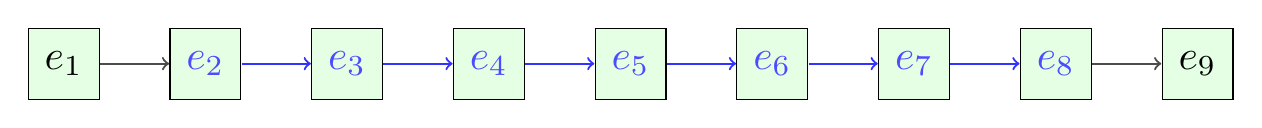
\begin{tikzpicture}[node distance = 0cm]
\node(num1)[num]{$\mathbi{e}_1$};
\node(num2)[num,right of = num1,xshift = 1.2cm]{\textcolor{blue!70}{$\mathbi{e}_2$}};
\node(num3)[num,right of = num2,xshift = 1.2cm]{\textcolor{blue!70}{$\mathbi{e}_3$}};
\node(num4)[num,right of = num3,xshift = 1.2cm]{\textcolor{blue!70}{$\mathbi{e}_4$}};
\node(num5)[num,right of = num4,xshift = 1.2cm]{\textcolor{blue!70}{$\mathbi{e}_5$}};
\node(num6)[num,right of = num5,xshift = 1.2cm]{\textcolor{blue!70}{$\mathbi{e}_6$}};
\node(num7)[num,right of = num6,xshift = 1.2cm]{\textcolor{blue!70}{$\mathbi{e}_7$}};
\node(num8)[num,right of = num7,xshift = 1.2cm]{\textcolor{blue!70}{$\mathbi{e}_8$}};
\node(num9)[num,right of = num8,xshift = 1.2cm]{$\mathbi{e}_9$};
%\node(A)[below of = num2,yshift = -0.6cm]{A};
%\node(B)[below of = num8,yshift = -0.6cm]{B};


\draw [->, thick, color = blue!80](num2.east)--(num3.west);
\draw [->, thick, color = blue!80](num3.east)--(num4.west);
\draw [->, thick, color = blue!80](num4.east)--(num5.west);
\draw [->, thick, color = blue!80](num5.east)--(num6.west);
\draw [->, thick, color = blue!80](num6.east)--(num7.west);
\draw [->, thick, color = blue!80](num7.east)--(num8.west);

\draw [->,thick,color = black!70] (num1) -- (num2);
\draw [->,thick,color =black!70] (num8) -- (num9);


\end{tikzpicture}}
\subfigure[卷积神经网络的层级结构]{\tikzstyle{num} = [rectangle, minimum width = 0.6cm, minimum height = 0.6cm, text centered,align=center,thick,draw = black,rounded corners=1.5pt]


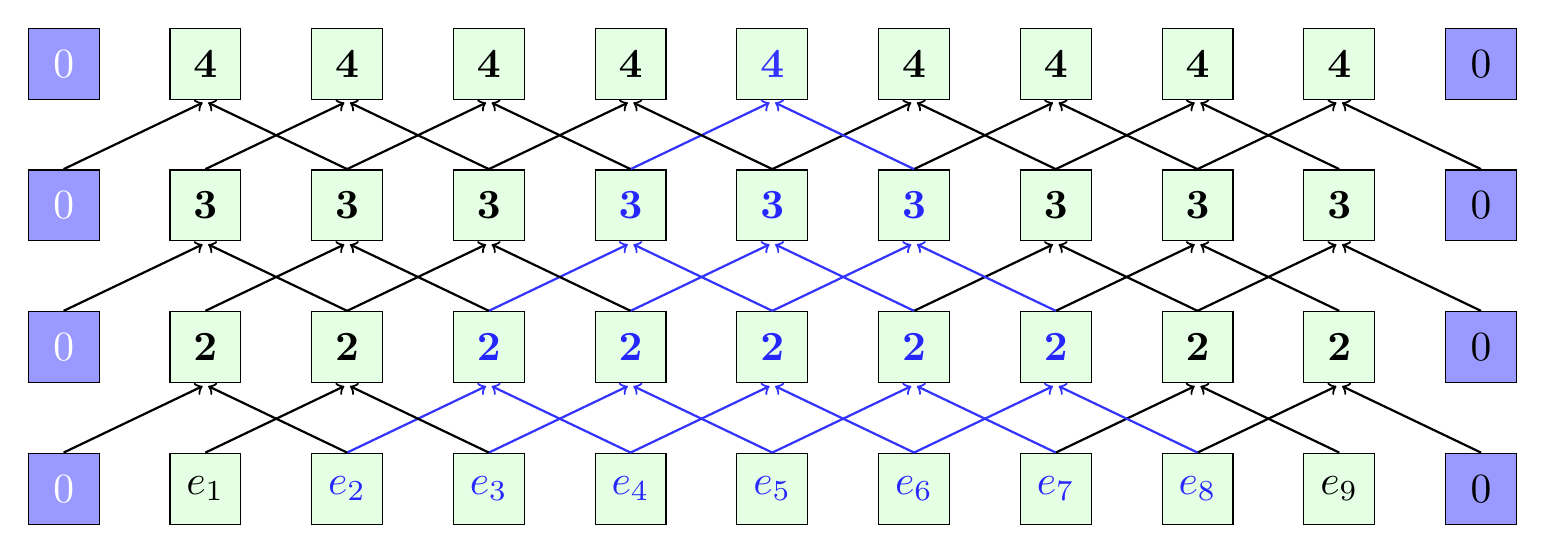
\begin{tikzpicture}[node distance = 0cm]
\node(num1_0)[num, fill = blue!40]{\textcolor{white}{$\mathbi{0}$}};
\node(num1_1)[num,right of = num1_0,xshift = 1.2cm]{$\mathbi{e}_1$};
\node(num1_2)[num,right of = num1_1,xshift = 1.2cm]{\textcolor{blue!85}{$\mathbi{e}_2$}};
\node(num1_3)[num,right of = num1_2,xshift = 1.2cm]{\textcolor{blue!85}{$\mathbi{e}_3$}};
\node(num1_4)[num,right of = num1_3,xshift = 1.2cm]{\textcolor{blue!85}{$\mathbi{e}_4$}};
\node(num1_5)[num,right of = num1_4,xshift = 1.2cm]{\textcolor{blue!85}{$\mathbi{e}_5$}};
\node(num1_6)[num,right of = num1_5,xshift = 1.2cm]{\textcolor{blue!85}{$\mathbi{e}_6$}};
\node(num1_7)[num,right of = num1_6,xshift = 1.2cm]{\textcolor{blue!85}{$\mathbi{e}_7$}};
\node(num1_8)[num,right of = num1_7,xshift = 1.2cm]{\textcolor{blue!85}{$\mathbi{e}_8$}};
\node(num1_9)[num,right of = num1_8,xshift = 1.2cm]{$\mathbi{e}_9$};
\node(num1_10)[num,right of = num1_9,xshift = 1.2cm, fill = blue!40]{$\mathbi{0}$};
%\node(A)[below of = num2,yshift = -0.6cm]{A};
%\node(B)[below of = num8,yshift = -0.6cm]{B};

\node(num2_0)[num,above of = num1_0,yshift = 1.2cm, fill = blue!40]{\textcolor{white}{$\mathbi{0}$}};
\node(num2_1)[num,right of = num2_0,xshift = 1.2cm]{\textbf2};
\node(num2_2)[num,right of = num2_1,xshift = 1.2cm]{\textbf2};
\node(num2_3)[num,right of = num2_2,xshift = 1.2cm]{\textbf{\textcolor{blue!85}2}};
\node(num2_4)[num,right of = num2_3,xshift = 1.2cm]{\textbf{\textcolor{blue!85}2}};
\node(num2_5)[num,right of = num2_4,xshift = 1.2cm]{\textbf{\textcolor{blue!85}2}};
\node(num2_6)[num,right of = num2_5,xshift = 1.2cm]{\textbf{\textcolor{blue!85}2}};
\node(num2_7)[num,right of = num2_6,xshift = 1.2cm]{\textbf{\textcolor{blue!85}2}};
\node(num2_8)[num,right of = num2_7,xshift = 1.2cm]{\textbf2};
\node(num2_9)[num,right of = num2_8,xshift = 1.2cm]{\textbf2};
\node(num2_10)[num,right of = num2_9,xshift = 1.2cm, fill = blue!40]{$\mathbi{0}$};

\node(num3_0)[num,above of = num2_0,yshift = 1.2cm, fill = blue!40]{\textcolor{white}{$\mathbi{0}$}};
\node(num3_1)[num,right of = num3_0,xshift = 1.2cm]{\textbf3};
\node(num3_2)[num,right of = num3_1,xshift = 1.2cm]{\textbf3};
\node(num3_3)[num,right of = num3_2,xshift = 1.2cm]{\textbf3};
\node(num3_4)[num,right of = num3_3,xshift = 1.2cm]{\textbf{\textcolor{blue!85}3}};
\node(num3_5)[num,right of = num3_4,xshift = 1.2cm]{\textbf{\textcolor{blue!85}3}};
\node(num3_6)[num,right of = num3_5,xshift = 1.2cm]{\textbf{\textcolor{blue!85}3}};
\node(num3_7)[num,right of = num3_6,xshift = 1.2cm]{\textbf3};
\node(num3_8)[num,right of = num3_7,xshift = 1.2cm]{\textbf3};
\node(num3_9)[num,right of = num3_8,xshift = 1.2cm]{\textbf3};
\node(num3_10)[num,right of = num3_9,xshift = 1.2cm, fill = blue!40]{$\mathbi{0}$};

\node(num4_0)[num,above of = num3_0,yshift = 1.2cm, fill = blue!40]{\textcolor{white}{$\mathbi{0}$}};
\node(num4_1)[num,right of = num4_0,xshift = 1.2cm]{\textbf4};
\node(num4_2)[num,right of = num4_1,xshift = 1.2cm]{\textbf4};
\node(num4_3)[num,right of = num4_2,xshift = 1.2cm]{\textbf4};
\node(num4_4)[num,right of = num4_3,xshift = 1.2cm]{\textbf4};
\node(num4_5)[num,right of = num4_4,xshift = 1.2cm]{\textbf{\textcolor{blue!80}4}};
\node(num4_6)[num,right of = num4_5,xshift = 1.2cm]{\textbf4};
\node(num4_7)[num,right of = num4_6,xshift = 1.2cm]{\textbf4};
\node(num4_8)[num,right of = num4_7,xshift = 1.2cm]{\textbf4};
\node(num4_9)[num,right of = num4_8,xshift = 1.2cm]{\textbf4};
\node(num4_10)[num,right of = num4_9,xshift = 1.2cm, fill = blue!40]{$\mathbi{0}$};

\draw [->, thick](num1_0.north)--([xshift=-0.1em,yshift=-0.1em]num2_1.south);
\draw [->, thick](num2_0.north)--([xshift=-0.1em,yshift=-0.1em]num3_1.south);
\draw [->, thick](num3_0.north)--([xshift=-0.1em,yshift=-0.1em]num4_1.south);
\draw [->, thick](num1_1.north)--([xshift=-0.1em,yshift=-0.1em]num2_2.south);
\draw [->, thick](num2_1.north)--([xshift=-0.1em,yshift=-0.1em]num3_2.south);
\draw [->, thick](num3_1.north)--([xshift=-0.1em,yshift=-0.1em]num4_2.south);
\draw [->, thick, color = blue!80](num1_2.north)--([xshift=-0.1em,yshift=-0.1em]num2_3.south);
\draw [->, thick](num2_2.north)--([xshift=-0.1em,yshift=-0.1em]num3_3.south);
\draw [->, thick](num3_2.north)--([xshift=-0.1em,yshift=-0.1em]num4_3.south);
\draw [->, thick, color = blue!80](num1_3.north)--([xshift=-0.1em,yshift=-0.1em]num2_4.south);
\draw [->, thick, color = blue!80](num2_3.north)--([xshift=-0.1em,yshift=-0.1em]num3_4.south);
\draw [->, thick](num3_3.north)--([xshift=-0.1em,yshift=-0.1em]num4_4.south);
\draw [->, thick, color = blue!80](num1_4.north)--([xshift=-0.1em,yshift=-0.1em]num2_5.south);
\draw [->, thick, color = blue!80](num2_4.north)--([xshift=-0.1em,yshift=-0.1em]num3_5.south);
\draw [->, thick, color = blue!80](num3_4.north)--([xshift=-0.1em,yshift=-0.1em]num4_5.south);
\draw [->, thick, color = blue!80](num1_5.north)--([xshift=-0.1em,yshift=-0.1em]num2_6.south);
\draw [->, thick, color = blue!80](num2_5.north)--([xshift=-0.1em,yshift=-0.1em]num3_6.south);
\draw [->, thick](num3_5.north)--([xshift=-0.1em,yshift=-0.1em]num4_6.south);
\draw [->, thick, color = blue!80](num1_6.north)--([xshift=-0.1em,yshift=-0.1em]num2_7.south);
\draw [->, thick](num2_6.north)--([xshift=-0.1em,yshift=-0.1em]num3_7.south);
\draw [->, thick](num3_6.north)--([xshift=-0.1em,yshift=-0.1em]num4_7.south);
\draw [->, thick](num1_7.north)--([xshift=-0.1em,yshift=-0.1em]num2_8.south);
\draw [->, thick](num2_7.north)--([xshift=-0.1em,yshift=-0.1em]num3_8.south);
\draw [->, thick](num3_7.north)--([xshift=-0.1em,yshift=-0.1em]num4_8.south);
\draw [->, thick](num1_8.north)--([xshift=-0.1em,yshift=-0.1em]num2_9.south);
\draw [->, thick](num2_8.north)--([xshift=-0.1em,yshift=-0.1em]num3_9.south);
\draw [->, thick](num3_8.north)--([xshift=-0.1em,yshift=-0.1em]num4_9.south);

\draw [->, thick](num1_2.north)--([xshift=0.1em,yshift=-0.1em]num2_1.south);
\draw [->, thick](num2_2.north)--([xshift=0.1em,yshift=-0.1em]num3_1.south);
\draw [->, thick](num3_2.north)--([xshift=0.1em,yshift=-0.1em]num4_1.south);
\draw [->, thick](num1_3.north)--([xshift=0.1em,yshift=-0.1em]num2_2.south);
\draw [->, thick](num2_3.north)--([xshift=0.1em,yshift=-0.1em]num3_2.south);
\draw [->, thick](num3_3.north)--([xshift=0.1em,yshift=-0.1em]num4_2.south);
\draw [->, thick, color = blue!80](num1_4.north)--([xshift=0.1em,yshift=-0.1em]num2_3.south);
\draw [->, thick](num2_4.north)--([xshift=0.1em,yshift=-0.1em]num3_3.south);
\draw [->, thick](num3_4.north)--([xshift=0.1em,yshift=-0.1em]num4_3.south);
\draw [->, thick, color = blue!80](num1_5.north)--([xshift=0.1em,yshift=-0.1em]num2_4.south);
\draw [->, thick, color = blue!80](num2_5.north)--([xshift=0.1em,yshift=-0.1em]num3_4.south);
\draw [->, thick](num3_5.north)--([xshift=0.1em,yshift=-0.1em]num4_4.south);
\draw [->, thick, color = blue!80](num1_6.north)--([xshift=0.1em,yshift=-0.1em]num2_5.south);
\draw [->, thick, color = blue!80](num2_6.north)--([xshift=0.1em,yshift=-0.1em]num3_5.south);
\draw [->, thick, color = blue!80](num3_6.north)--([xshift=0.1em,yshift=-0.1em]num4_5.south);
\draw [->, thick, color = blue!80](num1_7.north)--([xshift=0.1em,yshift=-0.1em]num2_6.south);
\draw [->, thick, color = blue!80](num2_7.north)--([xshift=0.1em,yshift=-0.1em]num3_6.south);
\draw [->, thick](num3_7.north)--([xshift=0.1em,yshift=-0.1em]num4_6.south);
\draw [->, thick, color = blue!80](num1_8.north)--([xshift=0.1em,yshift=-0.1em]num2_7.south);
\draw [->, thick](num2_8.north)--([xshift=0.1em,yshift=-0.1em]num3_7.south);
\draw [->, thick](num3_8.north)--([xshift=0.1em,yshift=-0.1em]num4_7.south);
\draw [->, thick](num1_9.north)--([xshift=0.1em,yshift=-0.1em]num2_8.south);
\draw [->, thick](num2_9.north)--([xshift=0.1em,yshift=-0.1em]num3_8.south);
\draw [->, thick](num3_9.north)--([xshift=0.1em,yshift=-0.1em]num4_8.south);
\draw [->, thick](num1_10.north)--([xshift=0.1em,yshift=-0.1em]num2_9.south);
\draw [->, thick](num2_10.north)--([xshift=0.1em,yshift=-0.1em]num3_9.south);
\draw [->, thick](num3_10.north)--([xshift=0.1em,yshift=-0.1em]num4_9.south);
\end{tikzpicture}}
\caption{串行及层级结构对比($\mathbi{e}_i$表示词嵌入,$\mathbi{0}$表示$\mathbi{0}$向量,方框里的2、3、4表示层次编号)}
\label{fig:11-9}
\end{figure}
%----------------------------------------------

\parinterval 针对不定长序列,一种可行的方法是使用之前介绍过的循环神经网络,其本质也是基于权重共享的想法,在不同的时间步复用相同的循环神经网络单元进行处理。但是,循环神经网络最大的弊端在于每一时刻的计算都依赖于上一时刻的结果,因此只能对序列进行串行处理,无法充分利用硬件设备进行并行计算,导致效率相对较低。此外,在处理较长的序列时,这种串行的方式很难捕捉长距离的依赖关系。相比之下,卷积神经网络采用共享参数的方式处理固定大小窗口内的信息,且不同位置的卷积操作之间没有相互依赖,因此可以对序列进行高效地并行处理。同时,针对序列中距离较长的依赖关系,可以通过堆叠多层卷积层来扩大{\small\bfnew{感受野}}\index{感受野} (Receptive Field)\index{Receptive Field}  ,这里感受野指能够影响神经元输出的原始输入数据区域的大小。图\ref{fig:11-9}对比了这两种结构,可以看出,为了捕捉$\mathbi{e}_2$ 和$\mathbi{e}_8$ 之间的联系,串行结构需要顺序的6次操作,和序列长度相关。而该卷积神经网络中,卷积操作每次对三个词进行计算,仅需要4层卷积计算就能得到$\mathbi{e}_2$ 和$\mathbi{e}_8$之间的联系,其操作数和卷积核的大小相关,相比于串行的方式具有更短的路径和更少的非线性计算,更容易进行训练。因此,也有许多研究人员在许多自然语言处理任务上尝试使用卷积神经网络进行序列建模\upcite{Kim2014ConvolutionalNN,Santos2014DeepCN,Kalchbrenner2014ACN,DBLP:conf/naacl/Johnson015,DBLP:conf/naacl/NguyenG15}。

\parinterval 区别于传统图像上的卷积操作,在面向序列的卷积操作中,卷积核只在序列这一维度进行移动,用来捕捉连续的多个词之间的特征。需要注意的是,由于单词通常由一个实数向量表示(词嵌入),因此可以将词嵌入的维度看作是卷积操作中的通道数。图\ref{fig:11-10}就是一个基于序列卷积的文本分类模型,模型的输入是维度大小为$m\times O $的句子表示,$m$表示句子长度,$O$表示卷积核通道数,其值等于词嵌入维度,模型使用多个不同(对应图中不同的颜色)的卷积核来对序列进行特征提取,得到了多个不同的特征序列。然后使用池化层降低表示维度,得到了一组和序列长度无关的特征表示。基于这组压缩过的特征表示,模型再通过全连接网络和Softmax函数作为相应类别的预测。在这其中卷积层和池化层分别起到了特征提取和特征压缩的作用,将一个不定长的序列转化到一组固定大小的特征表示。

%----------------------------------------------
% 图10.
\begin{figure}[htp]
\centering

%\newlength{\bcc}
\setlength{\bcc}{0.4cm}
\begin{tikzpicture}
\begin{scope}
	%\tikzstyle{every node}=[scale=0.8]
	\tikzstyle{line} = [dash pattern=on 2pt off 1pt,line width=0.6pt]
	\tikzstyle{cir} = [thin,fill=blue!8,draw,circle,minimum size =0.5em,drop shadow={shadow xshift=0.15em, shadow yshift=-0.1em}]
	\tikzstyle{word} = [inner sep=0pt, font=\footnotesize,minimum height=\bcc]
	
	%\draw[fill=blue!8,xshift=0.3cm,yshift=0.5cm,line width=0.6pt] (0cm,0cm) rectangle (0cm+6*\bcc,0cm+9*\bcc);
	%\draw[ugreen!60,step=\bcc,xshift=0.3cm,yshift=0.5cm,gray] (0cm,0cm) grid (0cm+6*\bcc,0cm+9*\bcc); 
	%\draw[red!60,line width=2pt,xshift=0.3cm,yshift=0.5cm] (0cm,0cm+2*\bcc) rectangle (0cm+6*\bcc,0cm+4*\bcc);
	
	% 输入矩阵
	\draw[thick,fill=blue!8,line width=0.6pt] (0cm,0cm) rectangle (0cm+6*\bcc,0cm+9*\bcc);
	\draw[step=\bcc,gray] (0cm,0cm) grid (0cm+6*\bcc,0cm+9*\bcc); 
	\draw[red!60,line width=2pt] (0cm,0cm) rectangle (0cm+6*\bcc,0cm+2*\bcc);
	\draw[ugreen!60,line width=2pt] (0cm,0cm+3*\bcc) rectangle (0cm+6*\bcc,0cm+6*\bcc);
	\draw[red!60,line width=2pt] (0cm,0cm+7*\bcc) rectangle (0cm+6*\bcc,0cm+9*\bcc);

	% 特征图
	\draw[fill=blue!8,xshift=5.0cm,yshift=1.3cm,line width=0.6pt] (0cm,0cm-1*\bcc) rectangle (0cm+1*\bcc,0cm+6*\bcc);
	\draw[step=\bcc,gray,xshift=5.0cm,yshift=1.3cm] (0cm,0cm-1*\bcc) grid (0cm+1*\bcc,0cm+6*\bcc);
	\draw[ugreen!60,line width=2pt,xshift=5.0cm,yshift=1.3cm] (0cm,0cm+2*\bcc) rectangle (0cm+1*\bcc,0cm+3*\bcc);
	
	%最大池化
	\draw [gray,fill=blue!8,line width=0.6pt](8cm,2.2cm) -- (8.4cm, 2.2cm) -- (8.7cm,1.4cm) -- (8.3cm, 1.4cm) -- (8cm,2.2cm);
	\draw [gray](8.15cm,1.8cm) -- (8.55cm,1.8cm);
	%\draw [gray](8.3cm,1.8cm) -- (8.7cm,1.8cm);
	%\draw [gray](8.45cm,1.4cm) -- (8.85cm,1.4cm);
	
	%全连接层
	\draw [gray,fill=blue!8,line width=0.6pt](11cm,2.2cm) -- (11.4cm, 2.2cm) -- (11.7cm,1.8cm) -- (11.3cm, 1.8cm) -- (11cm,2.2cm);
	%\draw [gray](11.15cm,1.8cm) -- (11.55cm,1.8cm);
	
	%最大池化
	\draw[ugreen!60,line] ([xshift=5.0cm,yshift=1.3cm]0cm+1*\bcc,0cm+6*\bcc) -- (8cm,2.2cm);
	\draw[ugreen!60,line] ([xshift=5.0cm,yshift=1.3cm]0cm+1*\bcc,0cm-1*\bcc) -- (8.15cm,1.8cm);

	%特征图
	%\draw[fill=blue!8,xshift=5.2cm,yshift=1.0cm,line width=0.6pt] (0cm,0cm) rectangle (0cm+1*\bcc,0cm+6*\bcc);
	%\draw[step=\bcc,gray,xshift=5.2cm,yshift=1.0cm] (0cm,0cm) grid (0cm+1*\bcc,0cm+6*\bcc); 
	
	%\draw[fill=blue!8,xshift=5.4cm,yshift=0.3cm,line width=0.6pt] (0cm,0cm) rectangle (0cm+1*\bcc,0cm+7*\bcc);
	%\draw[step=\bcc,gray,xshift=5.4cm,yshift=0.3cm] (0cm,0cm) grid (0cm+1*\bcc,0cm+7*\bcc);
	
	\draw[fill=blue!8,xshift=5.6cm,yshift=0cm,line width=0.6pt] (0cm,0cm) rectangle (0cm+1*\bcc,0cm+8*\bcc);
	\draw[step=\bcc,gray,xshift=5.6cm,yshift=0cm] (0cm,0cm) grid (0cm+1*\bcc,0cm+8*\bcc); 
	\draw[red!60,line width=2pt,xshift=5.6cm,yshift=0cm] (0cm,0cm) rectangle (0cm+1*\bcc,0cm+1*\bcc);
	\draw[red!60,line width=2pt,xshift=5.6cm,yshift=0cm] (0cm,0cm+7*\bcc) rectangle (0cm+1*\bcc,0cm+8*\bcc);
	
	% 全连接线
	\draw[line] (8.4cm, 2.2cm) -- (11.2cm,2.2cm);
	\draw[line] (8.7cm,1.4cm) -- (11.3cm, 1.8cm);
	%全连接上面的红虚线
	\draw[red!60,line] ([xshift=5.6cm,yshift=0cm]0cm+1*\bcc,0cm+7*\bcc) -- (8.15cm,1.8cm);
	\draw[red!60,line] ([xshift=5.6cm,yshift=0cm]0cm+1*\bcc,0cm) -- (8.3cm, 1.4cm);
	
	% 特征图红色虚线
	\draw[red!60,line] (0cm+6*\bcc,0cm+9*\bcc) -- ([xshift=5.6cm,yshift=0cm]0cm,0cm+8*\bcc);
	\draw[red!60,line] (0cm+6*\bcc,0cm+7*\bcc) -- ([xshift=5.6cm,yshift=0cm]0cm,0cm+7*\bcc);
	\draw[red!60,line] (0cm+6*\bcc,0cm+2*\bcc) -- ([xshift=5.6cm,yshift=0cm]0cm,0cm+1*\bcc);
	\draw[red!60,line] (0cm+6*\bcc,0cm) -- ([xshift=5.6cm,yshift=0cm]0cm,0cm);
	\draw[ugreen!60,line] (0cm+6*\bcc,0cm+6*\bcc) -- ([xshift=5.0cm,yshift=1.3cm]0cm,0cm+3*\bcc);
	\draw[ugreen!60,line] (0cm+6*\bcc,0cm+3*\bcc) -- ([xshift=5.0cm,yshift=1.3cm]0cm,0cm+2*\bcc);
	%\draw[red!60,line] ([xshift=0.3cm,yshift=0.5cm]0cm+6*\bcc,0cm+4*\bcc) -- ([xshift=5.6cm,yshift=0cm]0cm,0cm+3*\bcc);
	%\draw[red!60,line] ([xshift=0.3cm,yshift=0.5cm]0cm+6*\bcc,0cm+2*\bcc) -- ([xshift=5.6cm,yshift=0cm]0cm,0cm+2*\bcc);
	
	\node[word] (w1) at (-0.5cm, 3.4cm) {wait};
	\node[word] (w2) at ([yshift=-\bcc]w1) {for};
	\node[word] (w3) at ([yshift=-\bcc]w2) {the};
	\node[word] (w4) at ([yshift=-\bcc]w3) {video};
	\node[word] (w5) at ([yshift=-\bcc]w4) {and};
	\node[word] (w6) at ([yshift=-\bcc]w5) {do};
	\node[word] (w7) at ([yshift=-\bcc]w6) {n't};
	\node[word] (w8) at ([yshift=-\bcc]w7) {rent};
	\node[word] (w9) at ([yshift=-\bcc]w8) {it};
 
	\node[draw,rectangle callout,callout relative pointer={(0.28,-0.6)}] at (-0.3cm,4.6cm) {\textrm{卷积核}};
	\node[draw,rectangle callout,callout relative pointer={(0.1,-0.5)}] at (5cm,4.6cm) {\textrm{特征图}};


	\draw [thick] (0cm, -0.3cm) -- (0cm, -0.5cm)  -- node[font=\tiny, align=center,yshift=-0.5cm]{维度大小为 $m \times O$ \\ 的句子表示} (2.4cm,-0.5cm) -- (2.4cm, -0.3cm);	
	\draw [thick] (3.6cm, -0.3cm) -- (3.6cm, -0.5cm)  -- node[font=\tiny, align=center,yshift=-0.5cm]{具有多个不同大小\\的卷积核和特征图\\的卷积层} (6cm,-0.5cm) -- (6cm, -0.3cm);
	\draw [thick] (7.2cm, -0.3cm) -- (7.2cm, -0.5cm)  -- node[font=\tiny, align=center,yshift=-0.5cm]{最大池化} (9cm,-0.5cm) -- (9cm, -0.3cm);
	\draw [thick] (10cm, -0.3cm) -- (10cm, -0.5cm)  -- node[font=\tiny, align=center,yshift=-0.5cm]{带有Dropout\\和Softmax输出\\的全连接层} (11.7cm,-0.5cm) -- (11.7cm, -0.3cm);
	
	
\end{scope}

\end{tikzpicture}
\caption{序列卷积在文本分类模型中的应用\upcite{Kim2014ConvolutionalNN}}
\label{fig:11-10}
\end{figure}
%----------------------------------------------

\parinterval 和其它自然语言处理任务不同的是,机器翻译中需要对序列进行全局表示,换句话说,模型需要捕捉序列中各个位置之间的关系。因此,基于卷积神经网络的神经机器翻译模型需要堆叠多个卷积层进行远距离的依赖关系的建模。同时,为了在多层网络中维持序列的原有长度,需要在卷积操作前对输入序列进行填充。图\ref{fig:11-11}是一个简单的示例,针对一个长度$m=6$的句子,其隐层表示维度即卷积操作的输入通道数是$O=4$,卷积核大小为$K=3$。首先对序列进行填充,得到一个长度为8的序列,然后使用这些卷积核在这之上进行特征提取。一共使用了$N=4$个卷积核,整体的参数量为$K \times O \times N$,最后的卷积结果为$m \times N$的序列表示。

%----------------------------------------------
% 图11.
\begin{figure}[htp]
\centering
%\input{./Chapter11/Figures/figure-f }
%\newlength{\bcc}
\setlength{\bcc}{0.4cm}

\begin{tikzpicture}
\begin{scope}
	%\tikzstyle{every node}=[scale=0.8]
	\tikzstyle{line} = [dash pattern=on 2pt off 1pt,line width=0.5pt]
	\tikzstyle{cir} = [thin,fill=blue!8,draw,circle,minimum size =0.5em,drop shadow={shadow xshift=0.15em, shadow yshift=-0.1em}]
	\tikzstyle{word} = [inner sep=0pt, font=\scriptsize,minimum height=\bcc]
	
	\draw[fill=red!8,line width=0.2pt] (0cm,0cm+1*\bcc) rectangle (0cm+4*\bcc,0cm+7*\bcc);
	\draw[fill=cyan!14,line width=0.2pt] (0cm,0cm) rectangle (0cm+4*\bcc,0cm+1*\bcc);
	\draw[fill=cyan!14,line width=0.2pt] (0cm,0cm+7*\bcc) rectangle (0cm+4*\bcc,0cm+8*\bcc);
	\draw[step=\bcc] (0cm,0cm) grid (0cm+4*\bcc,0cm+8*\bcc); 
	%\draw[line width=0.7pt] (0cm,0cm) rectangle (0cm+4*\bcc,0cm+8*\bcc);
	\draw[red!50,line width=1.8pt] (0cm,0cm+5*\bcc) rectangle (0cm+4*\bcc,0cm+8*\bcc);
	\draw[ugreen!50,line width=1.8pt] (0cm,0cm+1*\bcc) rectangle (0cm+4*\bcc,0cm+4*\bcc);

	
	\draw[fill=blue!8,xshift=5.0cm,yshift=1.0cm,line width=0.2pt] (0cm,0cm) rectangle (0cm+1*\bcc,0cm+6*\bcc);
	\draw[step=\bcc,xshift=5.0cm,yshift=1.0cm] (0cm,0cm) grid (0cm+1*\bcc,0cm+6*\bcc);
	%\draw[line width=0.7pt,xshift=5.0cm,yshift=1.0cm] (0cm,0cm) rectangle (0cm+1*\bcc,0cm+6*\bcc);
	
	\draw[fill=blue!8,xshift=5.2cm,yshift=0.8cm,line width=0.2pt] (0cm,0cm) rectangle (0cm+1*\bcc,0cm+6*\bcc);
	\draw[step=\bcc,xshift=5.2cm,yshift=0.8cm] (0cm,0cm) grid (0cm+1*\bcc,0cm+6*\bcc); 
	%\draw[line width=0.7pt,xshift=5.2cm,yshift=0.8cm] (0cm,0cm) rectangle (0cm+1*\bcc,0cm+6*\bcc);
	\draw[ugreen!50,line width=2pt,xshift=5.2cm,yshift=0.8cm] (0cm,0cm+1*\bcc) rectangle (0cm+1*\bcc,0cm+2*\bcc);
	
	\draw[fill=blue!8,xshift=5.4cm,yshift=0.6cm,line width=0.2pt] (0cm,0cm) rectangle (0cm+1*\bcc,0cm+6*\bcc);
	\draw[step=\bcc,xshift=5.4cm,yshift=0.6cm] (0cm,0cm) grid (0cm+1*\bcc,0cm+6*\bcc);
	%\draw[line width=0.7pt,xshift=5.4cm,yshift=0.6cm] (0cm,0cm) rectangle (0cm+1*\bcc,0cm+6*\bcc); 
	
	\draw[fill=blue!8,xshift=5.6cm,yshift=0.4cm,line width=0.2pt] (0cm,0cm) rectangle (0cm+1*\bcc,0cm+6*\bcc);
	\draw[step=\bcc,xshift=5.6cm,yshift=0.4cm] (0cm,0cm) grid (0cm+1*\bcc,0cm+6*\bcc); 
	%\draw[line width=0.7pt,xshift=5.6cm,yshift=0.4cm] (0cm,0cm) rectangle (0cm+1*\bcc,0cm+6*\bcc);
	\draw[red!50,line width=2pt,xshift=5.6cm,yshift=0.4cm] (0cm,0cm+5*\bcc) rectangle (0cm+1*\bcc,0cm+6*\bcc);

	\draw[red!50,line width=0.5pt] (0cm+4*\bcc,0cm+8*\bcc) -- ([xshift=5.6cm,yshift=0.4cm]0cm,0cm+6*\bcc);
	\draw[red!50,line width=0.5pt] (0cm+4*\bcc,0cm+5*\bcc) -- ([xshift=5.6cm,yshift=0.4cm]0cm,0cm+5*\bcc);

	\draw[ugreen!50,line width=0.5pt] (0cm+4*\bcc,0cm+4*\bcc) -- ([xshift=5.2cm,yshift=0.8cm]0cm,0cm+2*\bcc);
	\draw[ugreen!50,line width=0.5pt] (0cm+4*\bcc,0cm+1*\bcc) -- ([xshift=5.2cm,yshift=0.8cm]0cm,0cm+1*\bcc);

	\node[word] (w1) at (-0.5cm, 3.0cm) {$<$p$>$};
	\node[word] (w2) at ([yshift=-\bcc]w1) {今天};
	\node[word] (w3) at ([yshift=-\bcc]w2) {是};
	\node[word] (w4) at ([yshift=-\bcc]w3) {个};
	\node[word] (w5) at ([yshift=-\bcc]w4) {好};
	\node[word] (w6) at ([yshift=-\bcc]w5) {日子};
	\node[word] (w7) at ([yshift=-\bcc]w6) {。};
	\node[word] (w8) at ([yshift=-\bcc]w7) {$<$p$>$};
	
	\node[inner xsep=2pt,inner ysep=0pt,font=\footnotesize] (c1) at (0.8cm, 3.5cm) {$O$};
	\draw[-latex] (c1.west) -- ([xshift=-0.4cm]c1.west);
	\draw[-latex] (c1.east) -- ([xshift=0.4cm]c1.east);
	
	\node[inner xsep=2pt,inner ysep=0pt,font=\footnotesize, rotate=-45] (c2) at (5.06cm, 0.5cm) {$N$};
	\draw[-latex] (c2.west) -- ([xshift=-0.2cm,yshift=0.2cm]c2.west);
	\draw[-latex] (c2.east) -- ([xshift=0.2cm, yshift=-0.2cm]c2.east);

%%%%%%%%%%%%%%%%%%%%%
	\node[word] (sub) at ([xshift=9.5*\bcc,yshift=3.5*\bcc]w1) {$O$\ \ :输入通道数};
	\node[word] (sub2) at ([yshift=-0.5*\bcc]sub.south) {$N$\ \ :卷积核数量};
	\node[word] (sub3) at ([xshift=-1.35em,yshift=-0.5*\bcc]sub2.south) {$<$p$>$:填充};
	
\end{scope}

\end{tikzpicture}
\caption{机器翻译中的序列卷积操作}
\label{fig:11-11}
\end{figure}
%----------------------------------------------

%----------------------------------------------------------------------------------------
%    NEW SECTION
%----------------------------------------------------------------------------------------
\sectionnewpage
\section{基于卷积神经网络的机器翻译模型}

\parinterval 正如之前所讲,卷积神经网络可以用于序列建模,同时具有并行性高和易于学习的特点,一个很自然的想法就是将其用作神经机器翻译模型中的特征提取器。因此,在神经机器翻译被提出之初,研究人员就已经开始利用卷积神经网络对句子进行特征提取。比较经典的模型是使用卷积神经网络作为源语言句子的编码器,使用循环神经网络作为目标语译文生成的解码器\upcite{kalchbrenner-blunsom-2013-recurrent,Gehring2017ACE}。之后也有研究人员提出完全基于卷积神经网络的翻译模型(ConvS2S)\upcite{DBLP:journals/corr/GehringAGYD17},或者针对卷积层进行改进,提出效率更高、性能更好的模型\upcite{Kaiser2018DepthwiseSC,Wu2019PayLA}。本节将基于ConvS2S模型,阐述如何使用卷积神经网络搭建端到端神经机器翻译模型。

%----------------------------------------------
% 图12.
\begin{figure}[htp]
\centering
%\documentclass[tikz]{standalone}
%\usepackage{tikz}
%\usepackage[UTF8]{ctex}
%\usetikzlibrary{shapes}
%\usetikzlibrary{backgrounds} 
%\usetikzlibrary{shadows}
%\usepackage{bm}
%\usetikzlibrary{fit}

\definecolor{mc_1_m}{RGB}{228,236,255}
\definecolor{mc_1}{RGB}{187,214,255}
\definecolor{mc_2_m}{RGB}{255,251,217}
\definecolor{mc_2}{RGB}{232,232,198}
\definecolor{mc_3_m}{RGB}{255,247,242}
\definecolor{mc_3}{RGB}{247,228,214}
\definecolor{mc_4_m}{RGB}{240,241,254}
\definecolor{mc_4}{RGB}{208,211,244}
\definecolor{ugreen}{rgb}{0,0.5,0}

\begin{tikzpicture}[scale=0.8]
	\tikzstyle{every node}=[scale=0.8]
	\tikzstyle{rec} = [thick,fill=red!10,draw,drop shadow,minimum height =1em,minimum width=2em]
	\tikzstyle{cir} = [line width=0.6pt,fill=yellow!20,draw,circle,minimum size =0.5em,drop shadow={shadow xshift=0.15em, shadow yshift=-0.1em}]
	\tikzstyle{word} = [inner sep=0pt, font=\footnotesize, minimum height=1em,align=center]
	
\begin{scope}
\foreach \point in {0,1,2,3,4,5}
\node[rec] (i_\point) at (0.9+\point, -0.1){};
\draw[thick] (i_0.0) -- (i_1.180);
\draw[thick] (i_1.0) -- (i_2.180);
\draw[thick] (i_2.0) -- (i_3.180);
\draw[thick] (i_3.0) -- (i_4.180);
\draw[thick] (i_4.0) -- (i_5.180);

\node[anchor=north,word] (tgt_1) at ([yshift=-0.4em]i_0.south){$<$p$>$};
\node[anchor=north,word] at ([yshift=-0.4em]i_1.south){$<$p$>$};
\node[anchor=north,word] at ([yshift=-0.4em]i_2.south){$<$sos$>$};
\node[anchor=north,word] at ([yshift=-0.4em]i_3.south){go};
\node[anchor=north,word] at ([yshift=-0.4em]i_4.south){to};
\node[anchor=north,word] (tgt_2) at ([yshift=-0.4em]i_5.south){school};

  \begin{pgfonlayer}{background}
	\node [draw=ugreen!30,rectangle,inner ysep=5pt,inner xsep=1.8em,rounded corners=4pt,line width=2pt,fill=ugreen!10] [fit = (tgt_1) (i_0)(tgt_2)(i_5) ] (group1_2) {};
  \end{pgfonlayer}

\node[anchor=east, word] (l_0) at ([xshift=-2em,yshift=-0.5em]i_0.west){\sffamily\bfnew{目标语词嵌入}};
\node[anchor=south, word] (l_1) at ([yshift=2em]l_0.north){\sffamily\bfnew{卷积}};
\node[anchor=south, word] (l_2) at ([yshift=2.4em]l_1.north){\sffamily\bfnew{门控}};
\node[anchor=south, word] (l_3) at ([yshift=0.06em]l_2.north){\sffamily\bfnew{线性单元}};


\foreach \point in {0,1,2}
\draw[thick,fill=blue!20] (5.9-\point,0.4) -- (4.9-\point,1.5) -- (3.9-\point,0.4) -- (5.9-\point,0.4);
\draw[thick,fill=blue!40] (2.9,0.4) -- (1.9,1.5) -- (0.9,0.4) -- (2.9,0.4);

\foreach \point in {0,1,2,3}{
\node[rec](h_\point) at (1.9+\point, 1.6){};
\draw[thick](h_\point.90) -- (h_\point.-90);
}

\foreach \point in {0,1,2,3}{
\node[cir](c_\point) at (1.7+\point, 2.4){};
\draw[out=20,in=160,line width=0.6pt] (c_\point.-135) to (c_\point.45);
\node[cir](x_\point) at (2.1+\point, 3){};
\draw[line width=0.6pt] (x_\point.-135) -- (x_\point.45);
\draw[line width=0.6pt] (x_\point.-45) -- (x_\point.135);
\draw[-latex,thick] ([xshift=-0.5em]h_\point.90) -- (c_\point.-90);
\draw[-latex,thick] ([xshift=0.5em]h_\point.90) -- (x_\point.-90);
\draw[-latex,out=90,in=-145,thick] (c_\point.90) to (x_\point.-145);
}

\foreach \point in {0,1,2,3}{
\node[rec](q_\point) at (2.5cm+\point*2em, 4){};
\draw[-latex,thick] (x_\point.90) -- (q_\point.-90);
}

\node[cir](o_1) at (7.55cm, 4){};
\draw[line width=0.6pt] (o_1.90) -- (o_1.-90);
\draw[line width=0.6pt] (o_1.0) -- (o_1.180);
\draw[-latex,thick] (q_3.0) -- (o_1.180);

\foreach \point in {0,1,2}{
\node[rec,fill=blue!40](g_\point_0) at (5cm+\point*2em, 7.5cm){};
\node[rec,fill=blue!40](g_\point_1) at (5cm+\point*2em, 7.5cm-1em){};
\node[rec,fill=blue!40](g_\point_2) at (5cm+\point*2em, 7.5cm-2em){};
\node[rec,fill=blue!40](g_\point_3) at (5cm+\point*2em, 7.5cm-3em){};
}

\node[anchor=north, word] at ([yshift=-0.6em]g_1_3.south){\sffamily\bfnew{内积}};

\draw [-latex, rounded corners=3pt,thick] (q_0.90) -- (2.5cm, 7.5cm) -- (g_0_0.180);
\draw [-latex, rounded corners=3pt,thick] (q_1.90) -- (2.5cm+2em, 7.5cm-1em) -- (g_0_1.180);
\draw [-latex, rounded corners=3pt,thick] (q_2.90) -- (2.5cm+4em, 7.5cm-2em) -- (g_0_2.180);
\draw [-latex, rounded corners=3pt,thick] (q_3.90) -- (2.5cm+6em, 6.2cm-2em) -- (2cm+6em, 6.2cm-2em) -- (2cm+6em, 7.5cm-3em) -- (g_0_3.180);
\node[thick,draw,fill=yellow!60,minimum height =1em,minimum width=2em](g_0_0) at (5cm, 7.5cm){};
\node[thick,draw,fill=yellow!60,minimum height =1em,minimum width=2em](g_1_1) at (5cm+2em, 7.5cm-1em){};
\node[thick,draw,fill=yellow!60,minimum height =1em,minimum width=2em](g_1_2) at (5cm+2em, 7.5cm-2em){};
\node[thick,draw,fill=yellow!60,minimum height =1em,minimum width=2em](g_2_3) at (5cm+4em, 7.5cm-3em){};

\foreach \point in {0,1,2,3}
\node[rec] (i_\point) at (8+\point, -0.1){};

\node[anchor=north,word] at ([yshift=-0.4em]i_0.south){go};
\node[anchor=north,word] at ([yshift=-0.4em]i_1.south){to};
\node[anchor=north,word] at ([yshift=-0.4em]i_2.south){school};
\node[anchor=north,word] at ([yshift=-0.4em]i_3.south){$<$eos$>$};

\foreach \point in {0,1,2,3}{
\node[cir,font=\fontsize{6}{6}\selectfont,inner sep=0.8pt](c_\point) at (8.2cm+\point*2em,7.5cm-1em*\point){\bm{$\sum$}};
\node[rec](q_\point) at (8.2cm+\point*2em, 5){};
\node[rec](b_\point) at (8.2cm+\point*2em, 4){};
\draw[-latex,thick] (g_2_\point.0) -- (c_\point.180);
\draw[-latex,thick] (c_\point.-90) -- (q_\point.90);
\draw[-latex,thick] (q_\point.-90) -- (b_\point.90);
\draw[-latex,thick] (b_\point.-90) -- ([yshift=-3.5cm]b_\point.-90);
}

\foreach \point in {2,1}
\draw[thick,fill=blue!20] (4.7cm+\point*1cm, 11cm) -- (3.9cm+\point*1cm, 12cm) -- (5.5cm+\point*1cm, 12cm) -- (4.7cm+\point*1cm, 11cm);
\draw[thick,fill=blue!40] (4.7cm,11cm) -- (3.9cm,12cm) -- (5.5cm,12cm) -- (4.7cm,11cm);

\foreach \point in {0,1,2}{
\node[rec](h_\point) at (5cm+\point*2em, 8.8cm){};
\node[rec](w_\point) at (8.6cm+\point*2em, 8.8cm){};
\node[cir](x_\point) at (4.5cm+\point*1cm, 9.6cm){};
\draw[line width=0.6pt] (x_\point.-135) -- (x_\point.45);
\draw[line width=0.6pt] (x_\point.-45) -- (x_\point.135);
\node[cir](c_\point) at (4.9cm+\point*1cm, 10.2cm){};
\draw[line width=0.6pt,out=20,in=160] (c_\point.-135) to (c_\point.45);
\node[rec](f_\point) at (4.7cm+\point*1cm, 11cm){};
\draw[-,thick] (f_\point.90) -- (f_\point.-90);
\draw[-latex,thick] ([xshift=-0.5em]f_\point.-90) -- (x_\point.90);
\draw[-latex,thick] ([xshift=0.5em]f_\point.-90) -- (c_\point.90);
\draw[-latex,out=-90,in=45,thick] (c_\point.-90) to (x_\point.45);
\draw[-latex,thick] (x_\point.-45) -- (h_\point.90);
\draw[-latex,thick] (h_\point.-90) -- (g_\point_0.90);
\node[rec](r_\point) at (4.7cm+\point*1cm, 12.55cm){};
}

\node[anchor=south,word] (src_1) at ([xshift=-2em,yshift=0.4em]r_0.north){$<$p$>$};
\node[anchor=south,word] at ([yshift=0.4em]r_0.north){去};
\node[anchor=south,word] at ([yshift=0.4em]r_1.north){上学};
\node[anchor=south,word] at ([yshift=0.4em]r_2.north){$<$sos$>$};
\node[anchor=south,word] (src_2) at ([xshift=2em,yshift=0.4em]r_2.north){$<$p$>$};


\node[anchor=east, word] (t_1) at ([xshift=-4em,yshift=0.5em]r_0.west){\sffamily\bfnew{源语词嵌入}};
\node[anchor=north, word] (t_2) at ([yshift=-2em]t_1.south){\sffamily\bfnew{卷积}};
\node[anchor=north, word] (t_3) at ([yshift=-2.8em]t_2.south){\sffamily\bfnew{门控}};
\node[anchor=north, word] (t_4) at ([yshift=-0.06em]t_3.south){\sffamily\bfnew{线性单元}};
\node[anchor=north, word] (t_5) at ([yshift=1.24em]t_4.south){\sffamily\bfnew{}};
\node[anchor=north, word] (t_6) at ([yshift=-1.5em]t_5.south){\sffamily\bfnew{注意力模块}};

\node[cir] (o_2) at (7.95, 8.8cm){};
\draw[line width=0.6pt] (o_2.90) -- (o_2.-90);
\draw[line width=0.6pt] (o_2.0) -- (o_2.180);
\draw[-latex,thick] (h_2.0) -- (o_2.180);
\node[cir] (o_3) at (8.6cm+2em, 10cm){};

\draw[thick] (r_0.0) -- (r_1.180);
\draw[thick] (r_1.0) -- (r_2.180);
\draw[rounded corners=3pt,thick] (r_2.0) -- (8.6cm+2em, 12.55cm) -- (o_3.90);
\draw[-latex,thick] (o_3.90) -- (o_3.-135) -- (w_0.90);
\draw[-latex,thick] (o_3.90) -- (o_3.-90) -- (w_1.90);
\draw[-latex,thick] (o_3.90) -- (o_3.-45) -- (w_2.90);

\node [single arrow,minimum height=2.4em,fill=blue!30,minimum width=4pt,rotate=-90,draw, fill=blue!20]  at (8.6cm+2em, 8cm) {};

  \begin{pgfonlayer}{background}
	\node [draw=ugreen!30,rectangle,inner ysep=5pt,inner xsep=1.3em,rounded corners=4pt,line width=2pt,fill=ugreen!10] [fit = (src_1) (src_2)(r_2) ] (group1_1) {};
	\node [rectangle,rounded corners=4pt,fill=mc_2_m, minimum width=3.8cm, minimum height=2.8cm]  (group2) at (5.7cm, 10.7cm) {};
	\node [rectangle,rounded corners=4pt,fill=mc_2_m, minimum width=5.2cm, minimum height=3.1cm]  (group3) at (3.4cm, 1.85cm) {};
	\draw [line width=2pt,draw=mc_1,fill=mc_1_m,rounded corners=4pt] ([yshift=0.4em,xshift=6em]t_6.north west) -- ([yshift=0.4em,xshift=6.3cm]t_6.north west) -- ([yshift=2.2cm,xshift=6.3cm]t_6.north west) --  ([yshift=2.2cm,xshift=9.8cm]t_6.north west) -- ([yshift=-5.4cm,xshift=9.8cm]t_6.north west) -- ([yshift=-5.4cm,xshift=-1.6em]t_6.north west)-- ([yshift=0.4em,xshift=-1.6em]t_6.north west) -- ([yshift=0.4em,xshift=6em]t_6.north west);
  \end{pgfonlayer}
\node [draw=mc_2!140,rectangle,rounded corners=4pt,line width=2pt,minimum width=3.8cm, minimum height=2.8cm] at (5.7cm, 10.7cm) {};
\node [draw=mc_2!140,rectangle,rounded corners=4pt,line width=2pt,minimum width=5.2cm, minimum height=3.1cm] at (3.4cm, 1.85cm) {};
\end{scope}

\end{tikzpicture} 
\caption{ConvS2S模型结构}
\label{fig:11-12}
\end{figure}
%----------------------------------------------

\parinterval ConvS2S模型是一种高并行的序列到序列的神经计算模型。该模型利用卷积神经网络分别对源语言端与目标语言端的序列进行特征提取,并使用注意力机制来捕获两个序列之间映射关系。相比于基于多层循环神经网络的GNMT模型\upcite{Wu2016GooglesNM},其主要优势在于每一层的网络计算是完全并行化的,避免了循环神经网络中计算顺序对时序的依赖。同时,利用多层卷积神经网络的层级结构可以有效地捕捉序列不同位置之间的依赖。即使是远距离依赖,也可以通过若干层卷积单元进行有效的捕捉,而且其信息传递的路径相比循环神经网络更短。除此之外,模型同时使用门控线性单元、残差网络和位置编码等技术来进一步提升模型性能,达到了和GNMT模型相媲美的翻译性能,同时大大缩短了训练时间。

\parinterval 图\ref{fig:11-12}为ConvS2S模型的结构示意图,其内部由若干不同的模块组成,包括:

\begin{itemize}
\item {\small\bfnew{位置编码}}\index{位置编码}(Position Embedding)\index{Position Embedding}:图中绿色背景框表示源语端词嵌入部分。相比于基于循环神经网络的翻译模型中的词嵌入,该模型还引入了位置编码,帮助模型获得词位置信息。位置编码具体实现在图\ref{fig:11-12}中没有显示,详见\ref{sec:11.2.1}节。

\item {\small\bfnew{卷积层}}与{\small\bfnew{门控线性单元}}(Gated Linear Units, GLU\index{Gated Linear Units, GLU}):黄色背景框是卷积模块,这里使用门控线性单元作为非线性函数,之前的研究工作\upcite{Dauphin2017LanguageMW} 表明这种非线性函数更适合于序列建模任务。图中为了简化,只展示了一层卷积,但在实际中为了更好地捕获句子信息,通常使用多层卷积的叠加。

\item {\small\bfnew{残差连接}}\index{残差连接}(Residual Connection)\index{Residual Connection}:对于源语言端和目标语言端的卷积层网络之间,都存在一个从输入到输出的额外连接,即跳接\upcite{DBLP:journals/corr/HeZRS15}。该连接方式确保每个隐层输出都能包含输入序列中的更多信息,同时能够有效提高深层网络的信息传递效率(该部分在图\ref{fig:11-12}中没有显示,具体结构详见\ref{sec:11.2.3}节)。

\item {\small\bfnew{多跳注意力机制}}\index{多跳注意力机制}(Multi-step Attention/Multi-hop Attention)\index{Multi-step Attention}\index{Multi-hop Attention}:蓝色框内部展示了基于多跳结构的注意力机制模块\upcite{Sukhbaatar2015EndToEndMN}。ConvS2S模型同样使用注意力机制来捕捉两个序列之间不同位置的对应关系。区别于之前的做法,多跳注意力在解码端每一个层都会执行注意力操作。下面将以此模型为例对基于卷积神经网络的机器翻译模型进行介绍。
\end{itemize}

%----------------------------------------------------------------------------------------
%    NEW SUB-SECTION
%----------------------------------------------------------------------------------------

\subsection{位置编码}
\label{sec:11.2.1}

\parinterval 与基于循环神经网络的翻译模型类似,基于卷积神经网络的翻译模型同样用词嵌入序列来表示输入序列,记为$\seq{w}=\{\mathbi{w}_1,\mathbi{w}_2,...,\mathbi{w}_m\}$。序列$\seq{w}$ 是维度大小为$m \times d$的矩阵,第$i$个单词$\mathbi{w}_i$是维度为$d$的向量,其中$m$为序列长度,$d$为词嵌入向量维度。和循环神经网络不同的是,基于卷积神经网络的模型需要对每个输入单词位置进行表示。这是由于,在卷积神经网络中,受限于卷积核的大小,单层的卷积神经网络只能捕捉序列局部的相对位置信息。虽然多层的卷积神经网络可以扩大感受野,但是对全局的位置表示并不充分。而相较于基于卷积神经网络的模型,基于循环神经网络的模型按时间步对输入的序列进行建模,这样间接的对位置信息进行了建模。而词序又是自然语言处理任务中重要信息,因此这里需要单独考虑。

\parinterval 为了更好地引入序列的词序信息,该模型引入了位置编码$\seq{p}=\{\mathbi{p}_1,\mathbi{p}_2,...,\mathbi{p}_m\}$,其中$\mathbi{p}_i$的维度大小为$d$,一般和词嵌入维度相等,其中具体数值作为网络可学习的参数。简单来说,$\mathbi{p}_i$是一个可学习的参数向量,对应位置$i$的编码。这种编码的作用就是对位置信息进行表示,不同序列中的相同位置都对应一个唯一的位置编码向量。之后将词嵌入矩阵和位置编码进行相加,得到模型的输入序列$\seq{e}=\{\mathbi{w}_1+\mathbi{p}_1,\mathbi{w}_2+\mathbi{p}_2,...,\mathbi{w}_m+\mathbi{p}_m\}$。 也有研究人员发现卷积神经网络本身具备一定的编码位置信息的能力\upcite{Islam2020HowMP},而这里额外的位置编码模块可以被看作是对卷积神经网络位置编码能力的一种补充。

%----------------------------------------------------------------------------------------
%    NEW SUB-SECTION
%----------------------------------------------------------------------------------------

\subsection{门控卷积神经网络}

\parinterval 单层卷积神经网络的感受野受限于卷积核的大小,因此只能捕捉序列中局部的上下文信息,不能很好地进行长序列建模。为了捕捉更长的上下文信息,最简单的做法就是堆叠多个卷积层。相比于循环神经网络的链式结构,对相同的上下文跨度,多层卷积神经网络的层级结构可以通过更少的非线性计算对其进行建模,缓解了长距离建模中的梯度消失问题。因此,卷积神经网络相对更容易进行训练。

%----------------------------------------------
% 图13.
\begin{figure}[htp]
\centering
%\documentclass[tikz]{standalone}
%\usepackage{tikz}
%\usepackage[UTF8]{ctex}
%\usetikzlibrary{shapes}
%\usetikzlibrary{backgrounds} 
%\usetikzlibrary{shadows}
%\usepackage{bm}
%\usetikzlibrary{fit}

\definecolor{mc_1_m}{RGB}{228,236,255}
\definecolor{mc_1}{RGB}{187,214,255}
\definecolor{mc_2_m}{RGB}{255,251,217}
\definecolor{mc_2}{RGB}{232,232,198}
\definecolor{mc_3_m}{RGB}{255,247,242}
\definecolor{mc_3}{RGB}{247,228,214}
\definecolor{mc_4_m}{RGB}{240,241,254}
\definecolor{mc_4}{RGB}{208,211,244}
\definecolor{ugreen}{rgb}{0,0.5,0}

\begin{tikzpicture}[scale=0.8]
	\tikzstyle{every node}=[scale=0.8]
	\tikzstyle{rec} = [thick,fill=red!10,draw,drop shadow,minimum height =1em,minimum width=2em]
	\tikzstyle{cir} = [line width=0.6pt,fill=yellow!20,draw,circle,minimum size =0.5em,drop shadow={shadow xshift=0.15em, shadow yshift=-0.1em}]
	\tikzstyle{word} = [inner sep=0pt, font=\footnotesize, minimum height=1em,align=center]
	
\begin{scope}
\foreach \point in {0,1,2,3,4,5}
\node[rec] (i_\point) at (0.9+\point, -0.1){};
\draw[thick] (i_0.0) -- (i_1.180);
\draw[thick] (i_1.0) -- (i_2.180);
\draw[thick] (i_2.0) -- (i_3.180);
\draw[thick] (i_3.0) -- (i_4.180);
\draw[thick] (i_4.0) -- (i_5.180);

\node[anchor=north,word] at ([yshift=-0.4em]i_0.south){$<$p$>$};
\node[anchor=north,word] at ([yshift=-0.4em]i_1.south){$<$p$>$};
\node[anchor=north,word] at ([yshift=-0.4em]i_2.south){$<$sos$>$};
\node[anchor=north,word] at ([yshift=-0.4em]i_3.south){go};
\node[anchor=north,word] at ([yshift=-0.4em]i_4.south){to};
\node[anchor=north,word] at ([yshift=-0.4em]i_5.south){school};

\node[anchor=east, word] (l_0) at ([xshift=-2em,yshift=-0.5em]i_0.west){\sffamily\bfnew{目标语词嵌入}};
\node[anchor=south, word] (l_1) at ([yshift=2em]l_0.north){\sffamily\bfnew{卷积}};
\node[anchor=south, word] (l_2) at ([yshift=2.4em]l_1.north){\sffamily\bfnew{门控}};
\node[anchor=south, word] (l_3) at ([yshift=0.06em]l_2.north){\sffamily\bfnew{线性单元}};

\foreach \point in {0,1,2}
\draw[thick,fill=blue!20] (5.9-\point,0.4) -- (4.9-\point,1.5) -- (3.9-\point,0.4) -- (5.9-\point,0.4);
\draw[thick,fill=blue!40] (2.9,0.4) -- (1.9,1.5) -- (0.9,0.4) -- (2.9,0.4);

\foreach \point in {0,1,2,3}{
\node[rec](h_\point) at (1.9+\point, 1.6){};
\draw[thick](h_\point.90) -- (h_\point.-90);
}

\foreach \point in {0,1,2,3}{
\node[cir](c_\point) at (1.7+\point, 2.4){};
\draw[out=20,in=160,line width=0.6pt] (c_\point.-135) to (c_\point.45);
\node[cir](x_\point) at (2.1+\point, 3){};
\draw[line width=0.6pt] (x_\point.-135) -- (x_\point.45);
\draw[line width=0.6pt] (x_\point.-45) -- (x_\point.135);
\draw[-latex,thick] ([xshift=-0.5em]h_\point.90) -- (c_\point.-90);
\draw[-latex,thick] ([xshift=0.5em]h_\point.90) -- (x_\point.-90);
\draw[-latex,out=90,in=-145,thick] (c_\point.90) to (x_\point.-145);
}

\foreach \point in {0,1,2,3}{
\node[rec](q_\point) at (2.5cm+\point*2em, 4){};
\draw[-latex,thick] (x_\point.90) -- (q_\point.-90);
}

\node[cir](o_1) at (7.55cm, 4){};
\draw[line width=0.6pt] (o_1.90) -- (o_1.-90);
\draw[line width=0.6pt] (o_1.0) -- (o_1.180);
\draw[-latex,thick] (q_3.0) -- (o_1.180);

\foreach \point in {0,1,2}{
\node[rec,fill=blue!40](g_\point_0) at (5cm+\point*2em, 7.5cm){};
\node[rec,fill=blue!40](g_\point_1) at (5cm+\point*2em, 7.5cm-1em){};
\node[rec,fill=blue!40](g_\point_2) at (5cm+\point*2em, 7.5cm-2em){};
\node[rec,fill=blue!40](g_\point_3) at (5cm+\point*2em, 7.5cm-3em){};
}

\node[anchor=north, word] at ([yshift=-0.6em]g_1_3.south){\sffamily\bfnew{内积}};

\draw [-latex, rounded corners=3pt,thick] (q_0.90) -- (2.5cm, 7.5cm) -- (g_0_0.180);
\draw [-latex, rounded corners=3pt,thick] (q_1.90) -- (2.5cm+2em, 7.5cm-1em) -- (g_0_1.180);
\draw [-latex, rounded corners=3pt,thick] (q_2.90) -- (2.5cm+4em, 7.5cm-2em) -- (g_0_2.180);
\draw [-latex, rounded corners=3pt,thick] (q_3.90) -- (2.5cm+6em, 6.2cm-2em) -- (2cm+6em, 6.2cm-2em) -- (2cm+6em, 7.5cm-3em) -- (g_0_3.180);
\node[thick,draw,fill=yellow!60,minimum height =1em,minimum width=2em](g_0_0) at (5cm, 7.5cm){};
\node[thick,draw,fill=yellow!60,minimum height =1em,minimum width=2em](g_1_1) at (5cm+2em, 7.5cm-1em){};
\node[thick,draw,fill=yellow!60,minimum height =1em,minimum width=2em](g_1_2) at (5cm+2em, 7.5cm-2em){};
\node[thick,draw,fill=yellow!60,minimum height =1em,minimum width=2em](g_2_3) at (5cm+4em, 7.5cm-3em){};

\foreach \point in {0,1,2,3}
\node[rec] (i_\point) at (8+\point, -0.1){};

\node[anchor=north,word] at ([yshift=-0.4em]i_0.south){go};
\node[anchor=north,word] at ([yshift=-0.4em]i_1.south){to};
\node[anchor=north,word] at ([yshift=-0.4em]i_2.south){school};
\node[anchor=north,word] at ([yshift=-0.4em]i_3.south){$<$eos$>$};

\foreach \point in {0,1,2,3}{
\node[cir,font=\fontsize{6}{6}\selectfont,inner sep=0.8pt](c_\point) at (8.2cm+\point*2em,7.5cm-1em*\point){\bm{$\sum$}};
\node[rec](q_\point) at (8.2cm+\point*2em, 5){};
\node[rec](b_\point) at (8.2cm+\point*2em, 4){};
\draw[-latex,thick] (g_2_\point.0) -- (c_\point.180);
\draw[-latex,thick] (c_\point.-90) -- (q_\point.90);
\draw[-latex,thick] (q_\point.-90) -- (b_\point.90);
\draw[-latex,thick] (b_\point.-90) -- ([yshift=-3.5cm]b_\point.-90);
}

\foreach \point in {2,1}
\draw[thick,fill=blue!20] (4.7cm+\point*1cm, 11cm) -- (3.9cm+\point*1cm, 12cm) -- (5.5cm+\point*1cm, 12cm) -- (4.7cm+\point*1cm, 11cm);
\draw[thick,fill=blue!40] (4.7cm,11cm) -- (3.9cm,12cm) -- (5.5cm,12cm) -- (4.7cm,11cm);

\foreach \point in {0,1,2}{
\node[rec](h_\point) at (5cm+\point*2em, 8.8cm){};
\node[rec](w_\point) at (8.6cm+\point*2em, 8.8cm){};
\node[cir](x_\point) at (4.5cm+\point*1cm, 9.6cm){};
\draw[line width=0.6pt] (x_\point.-135) -- (x_\point.45);
\draw[line width=0.6pt] (x_\point.-45) -- (x_\point.135);
\node[cir](c_\point) at (4.9cm+\point*1cm, 10.2cm){};
\draw[line width=0.6pt,out=20,in=160] (c_\point.-135) to (c_\point.45);
\node[rec](f_\point) at (4.7cm+\point*1cm, 11cm){};
\draw[-,thick] (f_\point.90) -- (f_\point.-90);
\draw[-latex,thick] ([xshift=-0.5em]f_\point.-90) -- (x_\point.90);
\draw[-latex,thick] ([xshift=0.5em]f_\point.-90) -- (c_\point.90);
\draw[-latex,out=-90,in=45,thick] (c_\point.-90) to (x_\point.45);
\draw[-latex,thick] (x_\point.-45) -- (h_\point.90);
\draw[-latex,thick] (h_\point.-90) -- (g_\point_0.90);
\node[rec](r_\point) at (4.7cm+\point*1cm, 12.55cm){};
}

\node[anchor=south,word] (src_1) at ([xshift=-2em,yshift=0.4em]r_0.north){$<$p$>$};
\node[anchor=south,word] at ([yshift=0.4em]r_0.north){去};
\node[anchor=south,word] at ([yshift=0.4em]r_1.north){上学};
\node[anchor=south,word] at ([yshift=0.4em]r_2.north){$<$sos$>$};
\node[anchor=south,word] (src_2) at ([xshift=2em,yshift=0.4em]r_2.north){$<$p$>$};


\node[anchor=east, word] (t_1) at ([xshift=-4em,yshift=0.5em]r_0.west){\sffamily\bfnew{源语词嵌入}};
\node[anchor=north, word] (t_2) at ([yshift=-2em]t_1.south){\sffamily\bfnew{卷积}};
\node[anchor=north, word] (t_3) at ([yshift=-2.8em]t_2.south){\sffamily\bfnew{门控}};
\node[anchor=north, word] (t_4) at ([yshift=-0.06em]t_3.south){\sffamily\bfnew{线性单元}};
\node[anchor=north, word] (t_5) at ([yshift=1.24em]t_4.south){\sffamily\bfnew{}};
\node[anchor=north, word] (t_6) at ([yshift=-1.5em]t_5.south){\sffamily\bfnew{注意力模块}};

\node[cir] (o_2) at (7.95, 8.8cm){};
\draw[line width=0.6pt] (o_2.90) -- (o_2.-90);
\draw[line width=0.6pt] (o_2.0) -- (o_2.180);
\draw[-latex,thick] (h_2.0) -- (o_2.180);
\node[cir] (o_3) at (8.6cm+2em, 10cm){};

\draw[thick] (r_0.0) -- (r_1.180);
\draw[thick] (r_1.0) -- (r_2.180);
\draw[rounded corners=3pt,thick] (r_2.0) -- (8.6cm+2em, 12.55cm) -- (o_3.90);
\draw[-latex,thick] (o_3.90) -- (o_3.-135) -- (w_0.90);
\draw[-latex,thick] (o_3.90) -- (o_3.-90) -- (w_1.90);
\draw[-latex,thick] (o_3.90) -- (o_3.-45) -- (w_2.90);

\node [single arrow,minimum height=2.4em,fill=blue!30,minimum width=4pt,rotate=-90,draw, fill=blue!20]  at (8.6cm+2em, 8cm) {};

  \begin{pgfonlayer}{background}
	%\node [draw=ugreen!30,rectangle,inner ysep=5pt,inner xsep=1.3em,rounded corners=4pt,line width=2pt,fill=ugreen!10] [fit = (src_1) (src_2)(r_2) ] (group1) {};
	\node [rectangle,rounded corners=4pt,fill=mc_2_m, minimum width=3.8cm, minimum height=2.8cm]  (group2) at (5.7cm, 10.7cm) {};
	\node [rectangle,rounded corners=4pt,fill=mc_2_m, minimum width=5.2cm, minimum height=3.1cm]  (group3) at (3.4cm, 1.85cm) {};
	%\draw [line width=2pt,draw=mc_1,fill=mc_1_m,rounded corners=4pt] ([yshift=0.4em,xshift=6em]t_6.north west) -- ([yshift=0.4em,xshift=6.3cm]t_6.north west) -- ([yshift=2.2cm,xshift=6.3cm]t_6.north west) --  ([yshift=2.2cm,xshift=9.8cm]t_6.north west) -- ([yshift=-5.4cm,xshift=9.8cm]t_6.north west) -- ([yshift=-5.4cm,xshift=-1.6em]t_6.north west)-- ([yshift=0.4em,xshift=-1.6em]t_6.north west) -- ([yshift=0.4em,xshift=6em]t_6.north west);
  \end{pgfonlayer}
\node [draw=mc_2!140,rectangle,rounded corners=4pt,line width=2pt,minimum width=3.8cm, minimum height=2.8cm] at (5.7cm, 10.7cm) {};
\node [draw=mc_2!140,rectangle,rounded corners=4pt,line width=2pt,minimum width=5.2cm, minimum height=3.1cm] at (3.4cm, 1.85cm) {};
\end{scope}

\end{tikzpicture} 
\caption{门控卷积神经网络机制在模型中的位置(黄色背景框部分)}
\label{fig:11-13}
\end{figure}
%----------------------------------------------

\parinterval 在ConvS2S模型中,编码端和解码端分别使用堆叠的门控卷积神经网络对源语和目标语序列进行建模,在传统卷积神经网络的基础上引入了门控线性单元\upcite{Dauphin2017LanguageMW},通过门控机制对卷积输出进行控制,它在模型中的位置如图\ref{fig:11-13}黄色方框所示:

\parinterval 门控机制在{\chapterten}中介绍LSTM模型时已经提到过。在LSTM模型中,可以通过引入三个门控单元来控制信息流,使隐层状态能够获得长时间记忆。同时,门控单元的引入简化了不同时间步间状态更新的计算,只包括一些线性计算,缓解了长距离建模中梯度消失的问题。在多层卷积神经网络中,同样可以通过门控机制来起到相同的作用。

\parinterval 图\ref{fig:11-14}是单层门控卷积神经网络的基本结构,$\mathbi{x}\in \mathbb{R}^{m\times d}$为单层网络的输入,$\mathbi{y} \in \mathbb{R}^{m \times d}$为单层网络的输出,网络结构主要包括卷积计算和GLU非线性单元两部分。

%----------------------------------------------
% 图14.
\begin{figure}[htp]
\centering
\newlength{\bd}
\setlength{\bd}{0.4cm}

\begin{tikzpicture}
	%\tikzstyle{every node}=[scale=0.8]
	\tikzstyle{word} = [inner sep=0pt, font=\scriptsize,minimum height=\bd]
	
	%\draw[fill=blue!8,xshift=0.3cm,yshift=0.5cm,line width=0.2pt] (0cm,0cm) rectangle (0cm+6*\bd,0cm+9*\bd);
	\draw[fill=cyan!20] (0cm,0cm) -- (4*\bd,0cm) -- (4*\bd,8*\bd) -- (0cm, 8*\bd) -- (0cm,0cm);
	\draw[cyan,step=\bd,line width=0.8pt] (0cm,0cm) grid (0cm+4*\bd,0cm+8*\bd);
	\draw[fill=red!10] (0cm,1*\bd) -- (4*\bd,1*\bd) -- (4*\bd,7*\bd) -- (0cm, 7*\bd) -- (0cm,1*\bd);
	\draw[red!60,step=\bd,xshift=0cm,yshift=\bd, line width=0.8pt] (0cm, 0cm) grid (0cm+4*\bd,0cm+6*\bd);
	\draw[fill=ugreen!10] (7*\bd,\bd) -- (11*\bd,\bd) -- (11*\bd,7*\bd) -- (7*\bd, 7*\bd) -- (7*\bd,\bd);
	\draw[ugreen!70,step=\bd,xshift=7*\bd,yshift=\bd, line width=0.8pt] (0cm, 0cm) grid (0cm+4*\bd,0cm+6*\bd);
	\draw[fill=ugreen!10] (11.5*\bd,\bd) -- (15.5*\bd,\bd) -- (15.5*\bd,7*\bd) -- (11.5*\bd, 7*\bd) -- (11.5*\bd,\bd);
	\draw[ugreen!70,step=\bd,xshift=11.5*\bd,yshift=\bd, line width=0.8pt] (0cm, 0cm) grid (0cm+4*\bd,0cm+6*\bd);
	\draw[fill=blue!10] (18.5*\bd,\bd) -- (22.5*\bd,\bd) -- (22.5*\bd,7*\bd) -- (18.5*\bd, 7*\bd) -- (18.5*\bd,\bd);
	\draw[blue!60,step=\bd,xshift=18.5*\bd,yshift=\bd, line width=0.8pt] (0cm, 0cm) grid (0cm+4*\bd,0cm+6*\bd);
	
	
	\draw[-,line width=0.6pt] (4*\bd, 0.5*\bd) -- (5.5*\bd, 1.5*\bd) -- (4*\bd, 2.5*\bd);
	\draw[-,line width=0.6pt] (4*\bd, 1.5*\bd) -- (5.5*\bd, 2.5*\bd) -- (4*\bd, 3.5*\bd);
	\draw[-,line width=0.6pt] (4*\bd, 2.5*\bd) -- (5.5*\bd, 3.5*\bd) -- (4*\bd, 4.5*\bd);
	\draw[-,line width=0.6pt] (4*\bd, 3.5*\bd) -- (5.5*\bd, 4.5*\bd) -- (4*\bd, 5.5*\bd);
	\draw[-,line width=0.6pt] (4*\bd, 4.5*\bd) -- (5.5*\bd, 5.5*\bd) -- (4*\bd, 6.5*\bd);
	\draw[-,line width=0.6pt] (4*\bd, 5.5*\bd) -- (5.5*\bd, 6.5*\bd) -- (4*\bd, 7.5*\bd);
	
	\node[draw,dash pattern=on 2pt off 1pt, rounded corners=2pt,minimum width=1.74cm, minimum height=2.56cm, inner sep=0pt, line width=0.6pt] (a) at (9*\bd, 4*\bd){};
	\node[draw,dash pattern=on 2pt off 1pt, rounded corners=2pt,minimum width=1.74cm, minimum height=2.56cm, inner sep=0pt, line width=0.6pt] (b) at (13.5*\bd, 4*\bd){};
	
	\draw[-latex,thick] (5.5*\bd, 1.5*\bd) -- (7*\bd-0.1cm, 1.5*\bd);
	\draw[-latex,thick] (5.5*\bd, 2.5*\bd) -- (7*\bd-0.1cm, 2.5*\bd);
	\draw[-latex,thick] (5.5*\bd, 3.5*\bd) -- (7*\bd-0.1cm, 3.5*\bd);
	\draw[-latex,thick] (5.5*\bd, 4.5*\bd) -- (7*\bd-0.1cm, 4.5*\bd);
	\draw[-latex,thick] (5.5*\bd, 5.5*\bd) -- (7*\bd-0.1cm, 5.5*\bd);
	\draw[-latex,thick] (5.5*\bd, 6.5*\bd) -- (7*\bd-0.1cm, 6.5*\bd);
	
	\node[word] (w1) at (-0.5cm, 7.5*\bd) {$<$p$>$};
	\node[word] (w2) at ([yshift=-\bd]w1) {今天};
	\node[word] (w3) at ([yshift=-\bd]w2) {是};
	\node[word] (w4) at ([yshift=-\bd]w3) {个};
	\node[word] (w5) at ([yshift=-\bd]w4) {好};
	\node[word] (w6) at ([yshift=-\bd]w5) {日子};
	\node[word] (w7) at ([yshift=-\bd]w6) {。};
	\node[word] (w8) at ([yshift=-\bd]w7) {$<$p$>$};

	\node[inner sep=2pt,word,fill=green!10,draw=ugreen,dotted,very thick,minimum width=6em,align=center,minimum height=4em] (sub) at ([xshift=11cm,yshift=-0.1cm]w1.east) {
\begin{tabular}{r l}
$<$p$>$:& 填充 \\
 $\sigma$:& sigmoid函数 \\
$\otimes$: & 按位乘运算 \\
 *: &卷积计算
\end{tabular}};
% $<$p$>$:填充 \\ $\sigma$:sigmoid函数 \\ $\otimes$:按位乘运算 \\ *:卷积计算
	
	\node[circle, draw, minimum size=0.7em, inner sep=0.5pt,font=\footnotesize,fill=yellow!40] (c1) at ([yshift=1.2em]b.north) {$\sigma$};
	\node[circle, draw, minimum size=0.7em, inner sep=0.5pt,font=\footnotesize,fill=yellow!40] (c2) at ([xshift=1.5em]b.east) {};
	\draw[-] (c2.45) -- (c2.-135);
	\draw[-] (c2.135) -- (c2.-45);
	
	\draw[-, rounded corners=2pt,thick] (a.north) --  ([yshift=1.2em]a.north) -- (c1.west); 
	\draw[-latex, rounded corners=2pt,thick] (c1.east) -- ([xshift=3.4em]c1.east) -- (c2.north);
	\draw[-latex,thick] (b.east) -- (c2.west);
	\draw[-latex,thick] (c2.east) -- ([xshift=0.4cm]c2.east); 
	
	\node[inner sep=0pt, font=\tiny] at (0.75cm, -0.4cm) {$\mathbi{x}$};
	\node[inner sep=0pt, font=\tiny] at ([yshift=-0.8cm]a.south) {$\mathbi{A}=\mathbi{x} * \mathbi{W} + \mathbi{b}_{\mathbi{W}}$};
	\node[inner sep=0pt, font=\tiny] at ([yshift=-0.8cm]b.south) {$\mathbi{B}=\mathbi{x} * \mathbi{V} + \mathbi{b}_{\mathbi{V}}$};
	\node[inner sep=0pt, font=\tiny] at (8.2cm, -0.4cm) {$\mathbi{y}=\mathbi{A} \otimes \sigma(\mathbi{B})$};
	
\end{tikzpicture}
\caption{单层门控卷积神经网络结构}
\label{fig:11-14}
\end{figure}
%----------------------------------------------


\parinterval 如图所示,形式上,卷积操作可以分成两部分,分别使用两个卷积核来得到两个卷积结果,具体计算如公式\eqref{eq:11-3}和\eqref{eq:11-4}所示:
\begin{eqnarray}
\mathbi{A} & = & \mathbi{x} * \mathbi{W} + \mathbi{b}_\mathbi{W} \label{eq:11-3} \\
\mathbi{B} & = & \mathbi{x} * \mathbi{V} + \mathbi{b}_\mathbi{V} \label{eq:11-4}
\end{eqnarray}

\noindent 其中,$\mathbi{A},\mathbi{B}\in \mathbb{R}^d$,$\mathbi{W}\in \mathbb{R}^{K\times d \times d}$、$\mathbi{V}\in \mathbb{R}^{K\times d \times d}$、$\mathbi{b}_\mathbi{W}$,$\mathbi{b}_\mathbi{V} \in \mathbb{R}^d $,$\mathbi{W}$、$\mathbi{V}$在此表示卷积核,$\mathbi{b}_\mathbi{W}$,$\mathbi{b}_\mathbi{V}$为偏置矩阵。在卷积操作之后,引入非线性变换,具体计算如公式\eqref{eq:11-5}所示:
\begin{eqnarray}
\mathbi{y} & = & \mathbi{A} \otimes \sigma ( \mathbi{B} )
\label{eq:11-5}
\end{eqnarray}

\noindent 其中,$\sigma$为Sigmoid函数,$\otimes$为按位乘运算。Sigmoid将$\mathbi{B}$映射为0-1范围内的实数,用来充当门控。可以看到,门控卷积神经网络中核心部分就是$\sigma ( \mathbi{B} )$,通过这个门控单元来对卷积输出进行控制,确定保留哪些信息。同时,在梯度反向传播的过程中,这种机制使得不同层之间存在线性的通道,梯度传导更加简单,利于深层网络的训练。这种思想和\ref{sec:11.2.3}节将要介绍的残差网络也很类似。

\parinterval 在ConvS2S模型中,为了保证卷积操作之后的序列长度不变,需要对输入进行填充,这一点已经在之前的章节中讨论过了。因此,在编码端每一次卷积操作前,需要对序列的头部和尾部分别做相应的填充(如图\ref{fig:11-14}左侧部分)。而在解码端中,由于需要训练和解码的一致性,模型在训练过程中不能使用未来的信息,需要对未来信息进行屏蔽,也就是屏蔽掉当前译文单词右侧的译文信息。从实践角度来看,只需要对解码端输入序列的头部填充$K-1$ 个空元素,其中$K$为卷积核的宽度(图\ref{fig:11-15}展示了卷积核宽度$K$=3时,解码端对输入序列的填充情况,图中三角形表示卷积操作)。

%----------------------------------------------
% 图14-2.
\begin{figure}[htp]
\centering

\begin{tikzpicture}
	%\tikzstyle{every node}=[scale=0.8]
	\tikzstyle{word} = [inner sep=2pt, minimum size=0.6cm]
	
	\node[word, text=black,rounded corners=1.5pt] (a1) at (0,0){$<$p$>$};
	\node[word, anchor=west,  text=black,rounded corners=1.5pt] (a2) at ([xshift=0.8em]a1.east){$<$p$>$};
	\node[word, inner sep=1pt,anchor=west,rounded corners=1.5pt] (a3) at ([xshift=0.8em]a2.east){$<$sos$>$};
	\node[word, anchor=west,rounded corners=1.5pt] (a4) at ([xshift=0.8em]a3.east){A};
	\node[word, anchor=west,rounded corners=1.5pt] (a5) at ([xshift=0.8em]a4.east){B};
	\node[word, anchor=west,rounded corners=1.5pt] (a6) at ([xshift=0.8em]a5.east){C};
	\node[word, anchor=west,rounded corners=1.5pt] (a7) at ([xshift=0.8em]a6.east){D};
	
	\node[word, anchor=south,rounded corners=1.5pt] (b1) at ([yshift=3em]a3.north) {A};
	\node[word, anchor=south, rounded corners=1.5pt] (b2) at ([yshift=3em]a4.north) {B};
	\node[word, anchor=south,rounded corners=1.5pt] (b3) at ([yshift=3em]a5.north) {C};
	\node[word, anchor=south,rounded corners=1.5pt] (b4) at ([yshift=3em]a6.north) {D};
	\node[word, anchor=south,rounded corners=1.5pt] (b5) at ([yshift=3em]a7.north) {$<$eos$>$};
	
	\draw[fill=blue!10,draw=blue!10] ([yshift=0.05em]a1.north) -- ([yshift=0.05em]a3.north) -- ([yshift=-0.05em]b1.south) -- ([yshift=0.05em]a1.north);
	\draw[fill=blue!20,draw=blue!20] ([yshift=0.05em]a2.north) -- ([yshift=0.05em]a4.north) -- ([yshift=-0.05em]b2.south) -- ([yshift=0.05em]a2.north);
	\draw[fill=blue!30,draw=blue!30] ([yshift=0.05em]a3.north) -- ([yshift=0.05em]a5.north) -- ([yshift=-0.05em]b3.south) -- ([yshift=0.05em]a3.north);
	\draw[fill=blue!40,draw=blue!40] ([yshift=0.05em]a4.north) -- ([yshift=0.05em]a6.north) -- ([yshift=-0.05em]b4.south) -- ([yshift=0.05em]a4.north);
	\draw[fill=blue!50,draw=blue!50] ([yshift=0.05em]a5.north) -- ([yshift=0.05em]a7.north) -- ([yshift=-0.05em]b5.south) -- ([yshift=0.05em]a5.north);

\node[inner sep=2pt,word,fill=blue!5,draw=blue!60,dotted,very thick,align=center,font=\scriptsize] (sub) at ([xshift=2.3cm,yshift=-0.8cm]b5.east) {
\begin{tabular}{r l}
$<$p$>$:& 填充 \\
$<$sos$>$:& 序列的开始 \\
$<$eos$>$: & 序列的终止
\end{tabular}};

\node[] at ([xshift=-6em]a1.west) {};
	
\end{tikzpicture}
\caption{解码端的填充方法}
\label{fig:11-15}
\end{figure}
%----------------------------------------------

%----------------------------------------------------------------------------------------
%    NEW SUB-SECTION
%----------------------------------------------------------------------------------------

\subsection{残差网络}
\label{sec:11.2.3}

\parinterval 残差连接是一种训练深层网络的技术,其内容在{\chapternine}已经进行了介绍,即在多层神经网络之间通过增加直接连接的方式,从而将底层信息直接传递给上层。通过增加这样的直接连接,可以让不同层之间的信息传递更加高效,有利于深层神经网络的训练,其计算如公式\eqref{eq:11-6}所示:
\begin{eqnarray}
\mathbi{h}^{l+1} = F (\mathbi{h}^l) + \mathbi{h}^l
\label{eq:11-6}
\end{eqnarray}

\noindent 其中,$\mathbi{h}^l$表示$l$层神经网络的输入向量,${F} (\mathbi{h}^l)$是$l$层神经网络的运算。如果$l=2$,那么公式\eqref{eq:11-6}可以解释为:第3层的输入$\mathbi{h}^3$等于第2层的输出${F}(\mathbi{h}^2)$加上第2层的输入$\mathbi{h}^2$。

\parinterval 在ConvS2S中残差连接主要应用于门控卷积神经网络和多跳自注意力机制中,比如在编码器的多层门控卷积神经网络中,在每一层的输入和输出之间增加残差连接,具体的数学描述如公式\eqref{eq:11-7}所示:
\begin{eqnarray}
%\mathbi{h}_i^l = \funp{v} (\mathbi{W}^l [\mathbi{h}_{i-\frac{k}{2}}^{l-1},...,\mathbi{h}_{i+\frac{k}{2}}^{l-1}] + b_{\mathbi{W}}^l ) + \mathbi{h}_i^{l-1}
\mathbi{h}^{l+1} = \mathbi{A}^{l} \otimes \sigma ( \mathbi{B}^{l} ) + \mathbi{h}^{l}
\label{eq:11-7}
\end{eqnarray}


%----------------------------------------------------------------------------------------
%    NEW SUB-SECTION
%----------------------------------------------------------------------------------------

\subsection{多跳注意力机制}

\parinterval ConvS2S模型也采用了注意力机制来获取每个目标语位置相应的源语言上下文信息。其仍然沿用传统的点乘注意力机制\upcite{DBLP:journals/corr/LuongPM15},其中图\ref{fig:11-16}蓝色框代表了多跳自注意力机制在模型中的位置。

\parinterval 在基于循环神经网络的翻译模型中,注意力机制已经被广泛使用\upcite{bahdanau2014neural},并用于避免循环神经网络将源语言序列压缩成一个固定维度的向量表示带来的信息损失。另一方面,注意力同样能够帮助解码端区分源语言中不同位置对当前目标语言位置的贡献度,其具体的计算过程如公式\eqref{eq:11-8}和\eqref{eq:11-9}所示:

\begin{eqnarray}
\mathbi{C}_j &=& \sum_i \alpha_{i,j} \mathbi{h}_i \label{eq:11-8} \\
\alpha_{i,j} &=& \frac{ \textrm{exp}(\funp{a} (\mathbi{s}_{j-1},\mathbi{h}_i))  }{\sum_{i'} \textrm{exp}( \funp{a} (\mathbi{s}_{j-1},\mathbi{h}_{i'}))} \label{eq:11-9}
\end{eqnarray}

\noindent 其中,$\mathbi{h}_i$表示源语端第$i$个位置的隐层状态,即编码器在第$i$个位置的输出。$\mathbi{s}_j$表示目标端第$j$个位置的隐层状态。给定$\mathbi{s}_j$和$\mathbi{h}_i$,注意力机制通过函数$\funp{a}(\cdot)$计算目标语言表示$\mathbi{s}_j$与源语言表示$\mathbi{h}_i$之间的注意力权重$\alpha_{i,j}$,通过加权平均得到当前目标端位置所需的上下文表示$\mathbi{C}_j$。其中$\funp{a}(\cdot)$的具体计算方式在{\chapterten}已经详细讨论。

%----------------------------------------------
% 图16.
\begin{figure}[htp]
\centering
%\documentclass[tikz]{standalone}
%\usepackage{tikz}
%\usepackage[UTF8]{ctex}
%\usetikzlibrary{shapes}
%\usetikzlibrary{backgrounds} 
%\usetikzlibrary{shadows}
%\usepackage{bm}
%\usetikzlibrary{fit}

\definecolor{mc_1_m}{RGB}{228,236,255}
\definecolor{mc_1}{RGB}{187,214,255}
\definecolor{mc_2_m}{RGB}{255,251,217}
\definecolor{mc_2}{RGB}{232,232,198}
\definecolor{mc_3_m}{RGB}{255,247,242}
\definecolor{mc_3}{RGB}{247,228,214}
\definecolor{mc_4_m}{RGB}{240,241,254}
\definecolor{mc_4}{RGB}{208,211,244}
\definecolor{ugreen}{rgb}{0,0.5,0}

\begin{tikzpicture}[scale=0.8]
	\tikzstyle{every node}=[scale=0.8]
	\tikzstyle{rec} = [thick,fill=red!10,draw,drop shadow,minimum height =1em,minimum width=2em]
	\tikzstyle{cir} = [line width=0.6pt,fill=yellow!20,draw,circle,minimum size =0.5em,drop shadow={shadow xshift=0.15em, shadow yshift=-0.1em}]
	\tikzstyle{word} = [inner sep=0pt, font=\footnotesize, minimum height=1em,align=center]
	
\begin{scope}
\foreach \point in {0,1,2,3,4,5}
\node[rec] (i_\point) at (0.9+\point, -0.1){};
\draw[thick] (i_0.0) -- (i_1.180);
\draw[thick] (i_1.0) -- (i_2.180);
\draw[thick] (i_2.0) -- (i_3.180);
\draw[thick] (i_3.0) -- (i_4.180);
\draw[thick] (i_4.0) -- (i_5.180);

\node[anchor=north,word] at ([yshift=-0.4em]i_0.south){$<$p$>$};
\node[anchor=north,word] at ([yshift=-0.4em]i_1.south){$<$p$>$};
\node[anchor=north,word] at ([yshift=-0.4em]i_2.south){$<$sos$>$};
\node[anchor=north,word] at ([yshift=-0.4em]i_3.south){go};
\node[anchor=north,word] at ([yshift=-0.4em]i_4.south){to};
\node[anchor=north,word] at ([yshift=-0.4em]i_5.south){school};

\node[anchor=east, word] (l_0) at ([xshift=-2em,yshift=-0.5em]i_0.west){\sffamily\bfnew{目标语词嵌入}};
\node[anchor=south, word] (l_1) at ([yshift=2em]l_0.north){\sffamily\bfnew{卷积}};
\node[anchor=south, word] (l_2) at ([yshift=2.4em]l_1.north){\sffamily\bfnew{门控}};
\node[anchor=south, word] (l_3) at ([yshift=0.06em]l_2.north){\sffamily\bfnew{线性单元}};


\foreach \point in {0,1,2}
\draw[thick,fill=blue!20] (5.9-\point,0.4) -- (4.9-\point,1.5) -- (3.9-\point,0.4) -- (5.9-\point,0.4);
\draw[thick,fill=blue!40] (2.9,0.4) -- (1.9,1.5) -- (0.9,0.4) -- (2.9,0.4);

\foreach \point in {0,1,2,3}{
\node[rec](h_\point) at (1.9+\point, 1.6){};
\draw[thick](h_\point.90) -- (h_\point.-90);
}

\foreach \point in {0,1,2,3}{
\node[cir](c_\point) at (1.7+\point, 2.4){};
\draw[out=20,in=160,line width=0.6pt] (c_\point.-135) to (c_\point.45);
\node[cir](x_\point) at (2.1+\point, 3){};
\draw[line width=0.6pt] (x_\point.-135) -- (x_\point.45);
\draw[line width=0.6pt] (x_\point.-45) -- (x_\point.135);
\draw[-latex,thick] ([xshift=-0.5em]h_\point.90) -- (c_\point.-90);
\draw[-latex,thick] ([xshift=0.5em]h_\point.90) -- (x_\point.-90);
\draw[-latex,out=90,in=-145,thick] (c_\point.90) to (x_\point.-145);
}

\foreach \point in {0,1,2,3}{
\node[rec](q_\point) at (2.5cm+\point*2em, 4){};
\draw[-latex,thick] (x_\point.90) -- (q_\point.-90);
}

\node[cir](o_1) at (7.55cm, 4){};
\draw[line width=0.6pt] (o_1.90) -- (o_1.-90);
\draw[line width=0.6pt] (o_1.0) -- (o_1.180);
\draw[-latex,thick] (q_3.0) -- (o_1.180);

\foreach \point in {0,1,2}{
\node[rec,fill=blue!40](g_\point_0) at (5cm+\point*2em, 7.5cm){};
\node[rec,fill=blue!40](g_\point_1) at (5cm+\point*2em, 7.5cm-1em){};
\node[rec,fill=blue!40](g_\point_2) at (5cm+\point*2em, 7.5cm-2em){};
\node[rec,fill=blue!40](g_\point_3) at (5cm+\point*2em, 7.5cm-3em){};
}

\node[anchor=north, word] at ([yshift=-0.6em]g_1_3.south){\sffamily\bfnew{内积}};

\draw [-latex, rounded corners=3pt,thick] (q_0.90) -- (2.5cm, 7.5cm) -- (g_0_0.180);
\draw [-latex, rounded corners=3pt,thick] (q_1.90) -- (2.5cm+2em, 7.5cm-1em) -- (g_0_1.180);
\draw [-latex, rounded corners=3pt,thick] (q_2.90) -- (2.5cm+4em, 7.5cm-2em) -- (g_0_2.180);
\draw [-latex, rounded corners=3pt,thick] (q_3.90) -- (2.5cm+6em, 6.2cm-2em) -- (2cm+6em, 6.2cm-2em) -- (2cm+6em, 7.5cm-3em) -- (g_0_3.180);
\node[thick,draw,fill=yellow!60,minimum height =1em,minimum width=2em](g_0_0) at (5cm, 7.5cm){};
\node[thick,draw,fill=yellow!60,minimum height =1em,minimum width=2em](g_1_1) at (5cm+2em, 7.5cm-1em){};
\node[thick,draw,fill=yellow!60,minimum height =1em,minimum width=2em](g_1_2) at (5cm+2em, 7.5cm-2em){};
\node[thick,draw,fill=yellow!60,minimum height =1em,minimum width=2em](g_2_3) at (5cm+4em, 7.5cm-3em){};

\foreach \point in {0,1,2,3}
\node[rec] (i_\point) at (8+\point, -0.1){};

\node[anchor=north,word] at ([yshift=-0.4em]i_0.south){go};
\node[anchor=north,word] at ([yshift=-0.4em]i_1.south){to};
\node[anchor=north,word] at ([yshift=-0.4em]i_2.south){school};
\node[anchor=north,word] at ([yshift=-0.4em]i_3.south){$<$eos$>$};

\foreach \point in {0,1,2,3}{
\node[cir,font=\fontsize{6}{6}\selectfont,inner sep=0.8pt](c_\point) at (8.2cm+\point*2em,7.5cm-1em*\point){\bm{$\sum$}};
\node[rec](q_\point) at (8.2cm+\point*2em, 5){};
\node[rec](b_\point) at (8.2cm+\point*2em, 4){};
\draw[-latex,thick] (g_2_\point.0) -- (c_\point.180);
\draw[-latex,thick] (c_\point.-90) -- (q_\point.90);
\draw[-latex,thick] (q_\point.-90) -- (b_\point.90);
\draw[-latex,thick] (b_\point.-90) -- ([yshift=-3.5cm]b_\point.-90);
}

\foreach \point in {2,1}
\draw[thick,fill=blue!20] (4.7cm+\point*1cm, 11cm) -- (3.9cm+\point*1cm, 12cm) -- (5.5cm+\point*1cm, 12cm) -- (4.7cm+\point*1cm, 11cm);
\draw[thick,fill=blue!40] (4.7cm,11cm) -- (3.9cm,12cm) -- (5.5cm,12cm) -- (4.7cm,11cm);

\foreach \point in {0,1,2}{
\node[rec](h_\point) at (5cm+\point*2em, 8.8cm){};
\node[rec](w_\point) at (8.6cm+\point*2em, 8.8cm){};
\node[cir](x_\point) at (4.5cm+\point*1cm, 9.6cm){};
\draw[line width=0.6pt] (x_\point.-135) -- (x_\point.45);
\draw[line width=0.6pt] (x_\point.-45) -- (x_\point.135);
\node[cir](c_\point) at (4.9cm+\point*1cm, 10.2cm){};
\draw[line width=0.6pt,out=20,in=160] (c_\point.-135) to (c_\point.45);
\node[rec](f_\point) at (4.7cm+\point*1cm, 11cm){};
\draw[-,thick] (f_\point.90) -- (f_\point.-90);
\draw[-latex,thick] ([xshift=-0.5em]f_\point.-90) -- (x_\point.90);
\draw[-latex,thick] ([xshift=0.5em]f_\point.-90) -- (c_\point.90);
\draw[-latex,out=-90,in=45,thick] (c_\point.-90) to (x_\point.45);
\draw[-latex,thick] (x_\point.-45) -- (h_\point.90);
\draw[-latex,thick] (h_\point.-90) -- (g_\point_0.90);
\node[rec](r_\point) at (4.7cm+\point*1cm, 12.55cm){};
}

\node[anchor=south,word] (src_1) at ([xshift=-2em,yshift=0.4em]r_0.north){$<$p$>$};
\node[anchor=south,word] at ([yshift=0.4em]r_0.north){去};
\node[anchor=south,word] at ([yshift=0.4em]r_1.north){上学};
\node[anchor=south,word] at ([yshift=0.4em]r_2.north){$<$sos$>$};
\node[anchor=south,word] (src_2) at ([xshift=2em,yshift=0.4em]r_2.north){$<$p$>$};


\node[anchor=east, word] (t_1) at ([xshift=-4em,yshift=0.5em]r_0.west){\sffamily\bfnew{源语词嵌入}};
\node[anchor=north, word] (t_2) at ([yshift=-2em]t_1.south){\sffamily\bfnew{卷积}};
\node[anchor=north, word] (t_3) at ([yshift=-2.8em]t_2.south){\sffamily\bfnew{门控}};
\node[anchor=north, word] (t_4) at ([yshift=-0.06em]t_3.south){\sffamily\bfnew{线性单元}};
\node[anchor=north, word] (t_5) at ([yshift=1.24em]t_4.south){\sffamily\bfnew{}};
\node[anchor=north, word] (t_6) at ([yshift=-1.5em]t_5.south){\sffamily\bfnew{注意力模块}};

\node[cir] (o_2) at (7.95, 8.8cm){};
\draw[line width=0.6pt] (o_2.90) -- (o_2.-90);
\draw[line width=0.6pt] (o_2.0) -- (o_2.180);
\draw[-latex,thick] (h_2.0) -- (o_2.180);
\node[cir] (o_3) at (8.6cm+2em, 10cm){};

\draw[thick] (r_0.0) -- (r_1.180);
\draw[thick] (r_1.0) -- (r_2.180);
\draw[rounded corners=3pt,thick] (r_2.0) -- (8.6cm+2em, 12.55cm) -- (o_3.90);
\draw[-latex,thick] (o_3.90) -- (o_3.-135) -- (w_0.90);
\draw[-latex,thick] (o_3.90) -- (o_3.-90) -- (w_1.90);
\draw[-latex,thick] (o_3.90) -- (o_3.-45) -- (w_2.90);

\node [single arrow,minimum height=2.4em,fill=blue!30,minimum width=4pt,rotate=-90,draw, fill=blue!20]  at (8.6cm+2em, 8cm) {};

  \begin{pgfonlayer}{background}
	%\node [draw=ugreen!30,rectangle,inner ysep=5pt,inner xsep=1.3em,rounded corners=4pt,line width=2pt,fill=ugreen!10] [fit = (src_1) (src_2)(r_2) ] (group1) {};
	%\node [rectangle,rounded corners=4pt,fill=mc_2_m, minimum width=3.8cm, minimum height=2.8cm]  (group2) at (5.7cm, 10.7cm) {};
	%\node [rectangle,rounded corners=4pt,fill=mc_2_m, minimum width=5.2cm, minimum height=3.1cm]  (group3) at (3.4cm, 1.85cm) {};
	\draw [line width=2pt,draw=mc_1,fill=mc_1_m,rounded corners=4pt] ([yshift=0.4em,xshift=6em]t_6.north west) -- ([yshift=0.4em,xshift=6.3cm]t_6.north west) -- ([yshift=2.2cm,xshift=6.3cm]t_6.north west) --  ([yshift=2.2cm,xshift=9.8cm]t_6.north west) -- ([yshift=-5.4cm,xshift=9.8cm]t_6.north west) -- ([yshift=-5.4cm,xshift=-1.6em]t_6.north west)-- ([yshift=0.4em,xshift=-1.6em]t_6.north west) -- ([yshift=0.4em,xshift=6em]t_6.north west);
  \end{pgfonlayer}
%\node [draw=mc_2!140,rectangle,rounded corners=4pt,line width=2pt,minimum width=3.8cm, minimum height=2.8cm] at (5.7cm, 10.7cm) {};
%\node [draw=mc_2!140,rectangle,rounded corners=4pt,line width=2pt,minimum width=5.2cm, minimum height=3.1cm] at (3.4cm, 1.85cm) {};
\end{scope}

\end{tikzpicture} 
\caption{多跳自注意力机制在ConvS2S模型中的位置(蓝色背景框部分)}
\label{fig:11-16}
\end{figure}
%----------------------------------------------

\parinterval 在ConvS2S模型中,解码器同样采用堆叠的多层门控卷积网络来对目标语言进行序列建模。区别于编码器,解码器在每一层卷积网络之后引入了注意力机制,用来参考源语言信息。ConvS2S选用了点乘注意力,并且通过类似残差连接的方式将注意力操作的输入与输出同时作用于下一层计算,称为多跳注意力。其具体计算方式如公式\eqref{eq:11-10}所示:
\begin{eqnarray}
\alpha_{ij}^l = \frac{ \textrm{exp} (\mathbi{d}_{j}^l\mathbi{h}_i) }{\sum_{i^{'}=1}^m \textrm{exp} (\mathbi{d}_{j}^l\mathbi{h}_{i^{'}})}
\label{eq:11-10}
\end{eqnarray}

\noindent 不同于公式\eqref{eq:11-9}中使用的目标语端隐层表示$\mathbi{s}_{j-1}$,公式\eqref{eq:11-10}中的$\mathbi{d}_{j}^l$同时结合了$\mathbi{s}_{j}$的卷积计算结果和目标语端的词嵌入$\mathbi{g}_j$,其具体计算如公式\eqref{eq:11-11}和\eqref{eq:11-12}所示:
\begin{eqnarray}
\mathbi{d}_{j}^l &=& \mathbi{W}_{d}^{l} \mathbi{z}_{j}^{l} + \mathbi{b}_{d}^{l} + \mathbi{g}_j \label{eq:11-11} \\
\mathbi{z}_j^l &=& \textrm{Conv}(\mathbi{s}_j^l) \label{eq:11-12}
\end{eqnarray}

\noindent 其中,$\mathbi{z}_j^l$表示第$l$层卷积网络输出中第$j$个位置的表示,$\mathbi{W}_{d}^{l}$和$\mathbi{b}_{d}^{l}$是模型可学习的参数,$\textrm{Conv}(\cdot)$表示卷积操作。在获得第$l$层的注意力权重之后,就可以得到对应的一个上下文表示$\mathbi{C}_j^l$,具体计算如公式\eqref{eq:11-13}所示:
\begin{eqnarray}
\mathbi{C}_j^l = \sum_i \alpha_{ij}^l (\mathbi{h}_i + \mathbi{e}_i)
\label{eq:11-13}
\end{eqnarray}

\noindent 模型使用了更全面的源语言信息,同时考虑了源语言端编码表示$\mathbi{h}_i$以及词嵌入表示$\mathbi{e}_i$。在获得第$l$层的上下文向量$\mathbi{C}_j^l$后,模型将其与$\mathbi{z}_j^l$相加后送入下一层网络,这个过程可以被描述为公式\eqref{eq:11-14}:
\begin{eqnarray}
\mathbi{s}_j^{l+1} = \mathbi{C}_j^l + \mathbi{z}_j^l
\label{eq:11-14}
\end{eqnarray}

\noindent 与循环网络中的注意力机制相比,该机制能够帮助模型甄别已经考虑了哪些先前的输入。也就是说,多跳的注意力机制会考虑模型之前更关注哪些单词,并且之后层中执行多次注意力的“跳跃”。

%----------------------------------------------------------------------------------------
%    NEW SUB-SECTION
%----------------------------------------------------------------------------------------

\subsection{训练与推断}

\parinterval 与基于循环神经网络的翻译模型一致,ConvS2S模型会计算每个目标语言位置上不同单词的概率,并以交叉熵作为损失函数来衡量模型预测分布与标准分布之间的差异。同时,采用基于梯度的方法对网络中的参数进行更新(见{\chapternine})。

\parinterval ConvS2S模型应用了很多工程方面的调整,主要包括:
\begin{itemize}
\vspace{0.5em}
\item ConvS2S模型使用了{\small\bfnew{Nesterov加速梯度下降法}} \index{Nesterov加速梯度下降法}(Nesterov Accelerated Gradient,NAG)\index{Nesterov Accelerated Gradient,NAG},动量累计的系数设置为0.99,当梯度范数超过0.1时重新进行规范化\upcite{Sutskever2013OnTI};

\vspace{0.5em}
\item ConvS2S模型中设置学习率为0.25,每当模型在校验集上的困惑度不再下降时,便在每轮的训练后将学习率降低一个数量级,直至学习率小于一定的阈值(如0.0004)。
\vspace{0.5em}

\end{itemize}

\parinterval Nesterov加速梯度下降法和{\chapternine}介绍的Momentum梯度下降法类似,都使用了历史梯度信息,首先回忆一下Momentum梯度下降法,具体计算如公式\eqref{eq:11-15}和\eqref{eq:11-16}所示:
\begin{eqnarray}
\mathbi{w}_{t+1} & = &  \mathbi{w}_t - \alpha \mathbi{v}_t \label{eq:11-15} \\
\mathbi{v}_t & = & \beta \mathbi{v}_{t-1} + (1-\beta)\frac{\partial J(\mathbi{w}_t)}{\partial \mathbi{w}_t}  \label{eq:11-16}
\end{eqnarray}

\noindent 其中,$\mathbi{w}_t$表示第$t$步更新时的模型参数;$J(\mathbi{w}_t)$表示损失函数均值期望的估计;$\frac{\partial J(\mathbi{w}_t)}{\partial \mathbi{w}_t}$将指向$J(\mathbi{w}_t)$在$\mathbi{w}_t$处变化最大的方向,即梯度方向;$\alpha$ 为学习率;$\mathbi{v}_t$为损失函数在前$t-1$步更新中累积的梯度动量,利用超参数$\beta$控制累积的范围。

\parinterval 而在Nesterov加速梯度下降法中,使用的梯度不是来自于当前参数位置,而是按照之前梯度方向更新一小步的位置,以便于更好地“预测未来”,提前调整更新速率,因此,其动量的更新方式如公式\eqref{eq:11-17}:
\begin{eqnarray}
\mathbi{v}_t & = & \beta \mathbi{v}_{t-1} + (1-\beta)\frac{\partial J(\mathbi{w}_t)}{\partial (\mathbi{w}_{t} -\alpha \beta \mathbi{v}_{t-1} )}
\label{eq:11-17}
\end{eqnarray}

\parinterval Nesterov加速梯度下降法其实是利用了二阶导数的信息,因此可以做到“向前看”,加速收敛过程\upcite{Bengio2013AdvancesIO}。为了模型的稳定训练。ConvS2S模型也采用了一些网络正则化和参数初始化的策略,使得模型在前向计算和反向计算过程中方差尽可能保持一致。

\parinterval 此外,ConvS2S模型为了进一步提升训练效率及性能,还使用了小批量训练,即每次从样本中选择出一小部分数据进行训练。同时,ConvS2S模型中也使用了Dropout方法\upcite{JMLR:v15:srivastava14a}。除了在词嵌入层和解码器输出层应用Dropout外,ConvS2S模型还对卷积块的输入层应用了Dropout。

\parinterval ConvS2S模型的推断过程与第十章中描述的推断过程一样。其基本思想是:依靠源语言句子和前面已经生成的译文单词来预测下一个译文单词。这个过程也可以结合贪婪搜索或者束搜索等解码策略。

%----------------------------------------------------------------------------------------
%    NEW SECTION
%----------------------------------------------------------------------------------------
\sectionnewpage
\section{局部模型的改进}

\parinterval 在序列建模中,卷积神经网络可以通过参数共享,高效地捕捉局部上下文特征,如图\ref{fig:11-11}所示。但是通过进一步分析可以发现,在标准卷积操作中包括了不同词和不同通道之间两种信息的交互,每个卷积核都是对相邻词的不同通道进行卷积操作,参数量为$K \times O$,其中,$K$为卷积核大小,$O$为输入的通道数,即单词表示的维度大小。如果使用$N$个卷积核,得到$N$个特征(即输出通道数),总共的参数量为$K \times O \times N$。 这里涉及卷积核大小、输入通道数和输出通道数三个维度,因此计算复杂度较高。为了进一步提升计算效率,降低参数量,一些研究人员提出{\small\bfnew{深度可分离卷积}}\index{深度可分离卷积}(Depthwise Separable Convolution)\index{Depthwise Separable Convolution},将空间维度和通道间的信息交互分离成{\small\bfnew{深度卷积}}(Depthwise Convolution,也叫逐通道卷积)\index{逐通道卷积}\index{Depthwise Convolution} 和{\small\bfnew{逐点卷积}} \index{逐点卷积}(Pointwise Convolution)\index{Pointwise Convolution} 两部分\upcite{Chollet2017XceptionDL,Howard2017MobileNetsEC}。 除了直接将深度可分离卷积应用到神经机器翻译中\upcite{Kaiser2018DepthwiseSC},研究人员提出使用更高效的{\small\bfnew{轻量卷积}}\index{轻量卷积}(Lightweight Convolution)\index{Lightweight Convolution}和{\small\bfnew{动态卷积}}\index{动态卷积}(Dynamic Convolution)\index{Dynamic convolution}来进行不同词之间的特征提取\upcite{Wu2019PayLA}。本节将主要介绍这些改进的卷积操作。在后续章节中也会看到这些模型在神经机器翻译中的应用。

%----------------------------------------------------------------------------------------
%    NEW SUB-SECTION
%----------------------------------------------------------------------------------------

\subsection{深度可分离卷积}
\label{sec:11.3.1}

\parinterval 根据前面的介绍,可以看到卷积神经网络容易用于局部检测和处理位置不变的特征。对于特定的表达,比如地点、情绪等,使用卷积神经网络能达到不错的识别效果,因此它常被用在文本分类中\upcite{Kalchbrenner2014ACN,Kim2014ConvolutionalNN,DBLP:conf/naacl/Johnson015,DBLP:conf/acl/JohnsonZ17}。不过机器翻译所面临的情况更复杂,除了局部句子片段信息,我们还希望模型能够捕获句子结构、语义等信息。虽然单层卷积神经网络在文本分类中已经取得了很好的效果\upcite{Kim2014ConvolutionalNN},但是神经机器翻译等任务仍然需要有效的卷积神经网络。随着深度可分离卷积在机器翻译中的探索\upcite{Kaiser2018DepthwiseSC},更高效的网络结构被设计出来,获得了比ConvS2S模型更好的性能。

%----------------------------------------------
% 图17.
\begin{figure}[htp]
\centering

\begin{tikzpicture}
	\tikzstyle{every node}=[scale=1.5]
	\tikzstyle{unit} = [inner sep=0pt, minimum size=1em,draw,very thick]
	%, font=\scriptsize
	\tikzstyle{vuale} = [inner sep=0pt,font=\tiny]

	\begin{scope}
	\foreach \point in {0,1,2}{
	\node[unit] (l1_\point) at (0, 0+\point*1.5em){};
	\node[unit] (l2_\point) at (0, 6em+\point*1.5em){};
	\node[unit] (l3_\point) at (0, 12em+\point*1.5em){};
	
	\node[unit] (r1_\point) at (5em, 0+\point*1.5em){};
	\node[unit] (r2_\point) at (5em, 6em+\point*1.5em){};
	\node[unit] (r3_\point) at (5em, 12em+\point*1.5em){};
	}
	
	\foreach \point in {0,1,2}{
	\draw[line width=0.5pt, ugreen!80, -latex] (l1_\point.east) -- ([xshift=-0.1em,yshift=-0.1em]r2_0.west);
	\draw[line width=0.5pt, orange!80, -latex] (l1_\point.east) -- ([xshift=-0.1em,yshift=-0.1em]r2_1.west);
	\draw[line width=0.5pt, cyan!80, -latex] (l1_\point.east) -- ([xshift=-0.1em,yshift=-0.1em]r2_2.west);
	\draw[line width=0.5pt, ugreen!80, -latex] (l2_\point.east) -- ([xshift=0em,yshift=0.1em]r2_0.west);
	\draw[line width=0.5pt, orange!80, -latex] (l2_\point.east) -- ([xshift=0em,yshift=0.1em]r2_1.west);
	\draw[line width=0.5pt, cyan!80, -latex] (l2_\point.east) -- ([xshift=0em,yshift=0.1em]r2_2.west);
	
	\draw[line width=0.5pt, ugreen!80, -latex] (l2_\point.east) -- ([xshift=-0.1em,yshift=-0.1em]r3_0.west);
	\draw[line width=0.5pt, orange!80, -latex] (l2_\point.east) -- ([xshift=-0.1em,yshift=-0.1em]r3_1.west);
	\draw[line width=0.5pt, cyan!80, -latex] (l2_\point.east) -- ([xshift=-0.1em,yshift=-0.1em]r3_2.west);
	\draw[line width=0.5pt, ugreen!80, -latex] (l3_\point.east) -- ([xshift=0em,yshift=0.1em]r3_0.west);
	\draw[line width=0.5pt, orange!80, -latex] (l3_\point.east) -- ([xshift=0em,yshift=0.1em]r3_1.west);
	\draw[line width=0.5pt, cyan!80, -latex] (l3_\point.east) -- ([xshift=0em,yshift=0.1em]r3_2.west);
	}
	
	\node[vuale] at ([xshift=-0.9em]l1_1.west) {$\mathbi{x}_3$};
	\node[vuale] at ([xshift=-0.9em]l2_1.west) {$\mathbi{x}_2$};
	\node[vuale] at ([xshift=-0.9em]l3_1.west) {$\mathbi{x}_1$};
	\node[vuale] at ([xshift=0.9em]r1_1.east) {$\mathbi{z}_3$};
	\node[vuale] at ([xshift=0.9em]r2_1.east) {$\mathbi{z}_2$};
	\node[vuale] at ([xshift=0.9em]r3_1.east) {$\mathbi{z}_1$};
	
	\node (t1) at (2.5em, -1em) {\large{$\cdots$}};
	\node [anchor=north,font=\tiny,scale=1.1] at ([yshift=-0.2em]t1.south) {(a) 标准卷积};
	\end{scope}
	
	\begin{scope}[xshift=4cm]
	\foreach \point in {0,1,2}{
	\node[unit] (l1_\point) at (0, 0+\point*1.5em){};
	\node[unit] (l2_\point) at (0, 6em+\point*1.5em){};
	\node[unit] (l3_\point) at (0, 12em+\point*1.5em){};
	
	\node[unit] (r1_\point) at (5em, 0+\point*1.5em){};
	\node[unit] (r2_\point) at (5em, 6em+\point*1.5em){};
	\node[unit] (r3_\point) at (5em, 12em+\point*1.5em){};
	}
	
	\foreach \point in {1,2}{
	\draw[line width=0.5pt, ugreen!80, -latex] (l\point_0.east) -- (r2_0.west);
	\draw[line width=0.5pt, orange!80, -latex] (l\point_1.east) -- (r2_1.west);
	\draw[line width=0.5pt, cyan!80, -latex] (l\point_2.east) -- (r2_2.west);
	}
	
	\foreach \point in {2,3}{
	\draw[line width=0.5pt, ugreen!80, -latex] (l\point_0.east) -- (r3_0.west);
	\draw[line width=0.5pt, orange!80, -latex] (l\point_1.east) -- (r3_1.west);
	\draw[line width=0.5pt, cyan!80, -latex] (l\point_2.east) -- (r3_2.west);
	}
	
	\node[vuale] at ([xshift=-0.9em]l1_1.west) {$\mathbi{x}_3$};
	\node[vuale] at ([xshift=-0.9em]l2_1.west) {$\mathbi{x}_2$};
	\node[vuale] at ([xshift=-0.9em]l3_1.west) {$\mathbi{x}_1$};
	\node[vuale] at ([xshift=0.9em]r1_1.east) {$\mathbi{z}_3$};
	\node[vuale] at ([xshift=0.9em]r2_1.east) {$\mathbi{z}_2$};
	\node[vuale] at ([xshift=0.9em]r3_1.east) {$\mathbi{z}_1$};
	
	\node (t2) at (2.5em, -1em) {\large{$\cdots$}};
	\node [anchor=north,font=\tiny,scale=1.1] at ([yshift=-0.2em]t2.south) {(b) 深度卷积};
	\end{scope}
	
	\begin{scope}[xshift=8cm]
	\foreach \point in {0,1,2}{
	\node[unit] (l1_\point) at (0, 0+\point*1.5em){};
	\node[unit] (l2_\point) at (0, 6em+\point*1.5em){};
	\node[unit] (l3_\point) at (0, 12em+\point*1.5em){};
	
	\node[unit] (r1_\point) at (5em, 0+\point*1.5em){};
	\node[unit] (r2_\point) at (5em, 6em+\point*1.5em){};
	\node[unit] (r3_\point) at (5em, 12em+\point*1.5em){};
	}
	
	\foreach \point in {0,1,2}{
	\draw[line width=0.5pt, ugreen!80, -latex] (l1_\point.east) -- (r1_0.west);
	\draw[line width=0.5pt, ugreen!80, -latex] (l2_\point.east) -- (r2_0.west);
	\draw[line width=0.5pt, ugreen!80, -latex] (l3_\point.east) -- (r3_0.west);
	
	\draw[line width=0.5pt, orange!80, -latex] (l1_\point.east) -- (r1_1.west);
	\draw[line width=0.5pt, orange!80, -latex] (l2_\point.east) -- (r2_1.west);
	\draw[line width=0.5pt, orange!80,, -latex] (l3_\point.east) -- (r3_1.west);
	
	\draw[line width=0.5pt, cyan!80, -latex] (l1_\point.east) -- (r1_2.west);
	\draw[line width=0.5pt, cyan!80, -latex] (l2_\point.east) -- (r2_2.west);
	\draw[line width=0.5pt, cyan!80, -latex] (l3_\point.east) -- (r3_2.west);
	}
	
	\node[vuale] at ([xshift=-0.9em]l1_1.west) {$\mathbi{x}_3$};
	\node[vuale] at ([xshift=-0.9em]l2_1.west) {$\mathbi{x}_2$};
	\node[vuale] at ([xshift=-0.9em]l3_1.west) {$\mathbi{x}_1$};
	\node[vuale] at ([xshift=0.9em]r1_1.east) {$\mathbi{z}_3$};
	\node[vuale] at ([xshift=0.9em]r2_1.east) {$\mathbi{z}_2$};
	\node[vuale] at ([xshift=0.9em]r3_1.east) {$\mathbi{z}_1$};
	
	\node (t3) at (2.5em, -1em) {\large{$\cdots$}};
	\node [anchor=north,font=\tiny,scale=1.1] at ([yshift=-0.2em]t3.south) {(c) 逐点卷积};
	\end{scope}
	
\end{tikzpicture}
\caption{标准卷积、深度卷积和逐点卷积示意图}
\label{fig:11-17}
\end{figure}
%----------------------------------------------

\parinterval 深度可分离卷积由深度卷积和逐点卷积两部分结合而成\upcite{sifre2014rigid}。图\ref{fig:11-17}对比了标准卷积、深度卷积和逐点卷积,为了方便显示,图中只画出了部分连接。

\parinterval 给定输入序列表示$\seq{x} = \{ \mathbi{x}_1,\mathbi{x}_2,...,\mathbi{x}_m \}$,其中$m$为序列长度,$\mathbi{x}_i \in \mathbb{R}^{O} $ ,$O$ 即输入序列的通道数。为了获得与输入序列长度相同的卷积输出结果,首先需要进行填充。为了方便描述,这里在输入序列尾部填充 $K-1$ 个元素($K$为卷积核窗口的长度),其对应的卷积结果为$\seq{z} = \{ \mathbi{z}_1,\mathbi{z}_2,...,\mathbi{z}_m \}$。
在标准卷积中,若使用N表示卷积核的个数,也就是标准卷积输出序列的通道数,那么对于第$i$个位置的第$n$个通道$ \mathbi{z}_{i,n}^\textrm{\,std}$,其标准卷积具体计算如公式\eqref{eq:11-18}所示:
\begin{eqnarray}
\mathbi{z}_{i,n}^\textrm{\,std} = \sum_{o=1}^{O} \sum_{k=0}^{K-1} \mathbi{W}_{k,o,n}^\textrm{\,std} \mathbi{x}_{i+k,o}
\label{eq:11-18}
\end{eqnarray}

%在标准卷积中,$ \mathbi{z}^\textrm{\,std}$表示标准卷积的输出,$ \mathbi{z}_i^\textrm{\,std} \in \mathbb{R}^N$ ,N为卷积核的个数,也就是标准卷积输出序列的通道数。针对$ \mathbi{z}_i^\textrm{\,std} $ 中的第$n$个通道$ \mathbi{z}_{i,n}^\textrm{\,std}$,标准卷积具体计算方式如下:

\noindent 其中,$ \mathbi{z}^\textrm{\,std}$表示标准卷积的输出,$ \mathbi{z}_i^\textrm{\,std} \in \mathbb{R}^N$, $\mathbi{W}^\textrm{\,std} \in \mathbb{R}^{K \times O \times N} $ 为标准卷积的参数。可以看出,标准卷积中每个输出元素需要考虑卷积核尺度内所有词的所有特征,参数量相对较多,对应图\ref{fig:11-17}中的连接数也最多。

\parinterval 相应的,深度卷积只考虑不同词之间的依赖性,而不考虑不同通道之间的关系,相当于使用$O$个卷积核逐个通道对不同的词进行卷积操作。因此深度卷积不改变输出的表示维度,输出序列表示的通道数与输入序列一致,其计算如公式\eqref{eq:11-19}所示:
\begin{eqnarray}
\mathbi{z}_{i,o}^\textrm{\,dw} = \sum_{k=0}^{K-1} \mathbi{W}_{k,o}^\textrm{\,dw} \mathbi{x}_{i+k,o}
\label{eq:11-19}
\end{eqnarray}

\noindent 其中,$\mathbi{z}^\textrm{\,dw}$表示深度卷积的输出,$\mathbi{z}_i^\textrm{\,dw} \in \mathbb{R}^{O}$ ,$\mathbi{W}^\textrm{\,dw} \in \mathbb{R}^{K \times O}$为深度卷积的参数,参数量只涉及卷积核大小及输入表示维度。

\parinterval 与深度卷积互为补充的是,逐点卷积只考虑不同通道之间的依赖性,而不考虑不同词之间的依赖。换句话说,逐点卷积对每个词表示做了一次线性变换,将输入表示$\mathbi{x}_i$从 $\mathbb{R}^{O}$ 的空间映射到 $\mathbb{R}^{N}$的空间,其具体计算如公式\eqref{eq:11-20}所示:
\begin{eqnarray}
\mathbi{z}_{i,n}^\textrm{\,pw} &=& \sum\limits_{o=1}^{O} \mathbi{x}_{i,o} \mathbi{W}_{o,n}^\textrm{\,pw} \nonumber \\
                      &=& \mathbi{x}_i \mathbi{W}^\textrm{\,pw}
\label{eq:11-20}
\end{eqnarray}

\noindent 其中$\mathbi{z}^\textrm{\,pw}$表示逐点卷积的输出,$\mathbi{z}_{i}^\textrm{\,pw} \in  \mathbb{R}^{N}$,$\mathbi{W}^\textrm{\,pw} \in \mathbb{R}^{O \times N}$为逐点卷积的参数。

\parinterval 表\ref{tab:11-1}展示了这几种不同类型卷积的参数量,深度可分离卷积通过将标准卷积进行分解,降低了整体模型的参数量。在相同参数量的情况下,深度可分离卷积可以采用更大的卷积窗口,考虑序列中更大范围的依赖关系。因此相比于标准卷积,深度可分离卷积具有更强的表示能力,在机器翻译任务中也能获得更好的性能。

%----------------------------------------------
\begin{table}[htp]
\centering
\caption{不同类型卷积的参数量对比($K$表示卷积核大小,$O$表示输入通道数,$N$表示输出通道数)\upcite{StahlbergNeural}}
\label{tab:11-1}
\begin{tabular}{l | l}
卷积类型 & 参数量 \\ \hline
\rule{0pt}{12pt}标准卷积 & $K \times O \times N$ \\
深度卷积 & $K \times O$ \\
逐点卷积 & $O \times N$ \\
深度可分离卷积 & $K \times O + O \times N $
\end{tabular}
\end{table}
%----------------------------------------------

%----------------------------------------------------------------------------------------
%    NEW SUB-SECTION
%----------------------------------------------------------------------------------------

\subsection{轻量卷积和动态卷积}

\parinterval 深度可分离卷积中深度卷积的作用就是用来捕捉相邻词之间的依赖关系,这和{\chaptertwelve}即将介绍的基于自注意力机制的模型类似。基于深度卷积,一些研究人员提出了轻量卷积和动态卷积,用来替换注意力机制,并将其应用于基于自注意力机制的模型中\upcite{Wu2019PayLA}。同时,卷积操作的线性复杂度使得它具有较高的运算效率,相比注意力机制的平方复杂度,卷积操作是一种更加“轻量”的方法。接下来分别介绍轻量卷积与动态卷积的思想。

%----------------------------------------------------------------------------------------
%    NEW SUBSUB-SECTION
%----------------------------------------------------------------------------------------
\subsubsection{1. 轻量卷积}

\parinterval 在序列建模的模型中,一个很重要的模块就是对序列中不同位置信息的提取,如ConvS2S模型中的卷积神经网络等。虽然考虑局部上下文的卷积神经网络只在序列这一维度进行操作,具有线性的复杂度,但是由于标准卷积操作中考虑了不同通道的信息交互,整体复杂度依旧较高。一种简化的策略就是采取通道独立的卷积操作,也就是\ref{sec:11.3.1}节中介绍的深度卷积。

\parinterval 在神经机器翻译模型中,神经网络不同层的维度通常一致,即$O=N=d$。因此,深度卷积可以使得卷积神经网络参数量从 $Kd^2$ 降到$Kd$(参考表\ref{tab:11-1})。从形式上来看,深度卷积和注意力机制很类似,区别在于注意力机制考虑了序列全局上下文信息,权重来自于当前位置对其他位置的“注意力”,而深度卷积中仅考虑了局部的上下文信息,权重采用了在不同通道上独立的固定参数。为了进一步降低参数量,轻量卷积共享了部分通道的卷积参数。如图\ref{fig:11-18}所示,深度卷积中4种颜色的连接代表了4个通道上独立的卷积核,而轻量卷积中,第一和第三通道,第二和第四通道采用了共享的卷积核参数。通过共享,可以将参数量压缩到$Ka$,其中压缩比例为$d/a$($a$为压缩后保留的共享通道数)。

%----------------------------------------------
% 图18.
\begin{figure}[htp]
\centering

\begin{tikzpicture}
	\tikzstyle{every node}=[scale=1.5]
	\tikzstyle{unit} = [inner sep=0pt, minimum size=1em,draw,very thick]
	\tikzstyle{vuale} = [inner sep=0pt,font=\tiny]

	
	\begin{scope}
	\foreach \point in {0,1,2,3}{
	\node[unit] (l1_\point) at (0, 0+\point*1.5em){};
	\node[unit] (l2_\point) at (0, 8em+\point*1.5em){};
	
	\node[unit] (r1_\point) at (5em, 0+\point*1.5em){};
	\node[unit] (r2_\point) at (5em, 8em+\point*1.5em){};
	}
	
	\foreach \point in {1,2}{
	\draw[line width=0.9pt, ugreen!80, -latex] (l\point_0.east) -- (r2_0.west);
	\draw[line width=0.9pt, orange!80, -latex] (l\point_1.east) -- (r2_1.west);
	\draw[line width=0.9pt, cyan!80, -latex] (l\point_2.east) -- (r2_2.west);
	\draw[line width=0.9pt, gray!80, -latex] (l\point_3.east) -- (r2_3.west);
	}
	
	\node[vuale] at (-1.5em, 1.9em) {$\mathbi{x}_2$};
	\node[vuale] at (-1.5em, 9.9em) {$\mathbi{x}_1$};
	\node[vuale] at (6.5em, 1.9em) {$\mathbi{z}_2$};
	\node[vuale] at (6.5em, 9.9em) {$\mathbi{z}_1$};
	
	\node (t2) at (2.5em, -1em) {\large{$\cdots$}};
	\node [anchor=north,font=\tiny] at ([yshift=-0.2em]t2.south) {深度卷积};
	\end{scope}

	\begin{scope}[xshift=4cm]
	\foreach \point in {0,1,2,3}{
	\node[unit] (l1_\point) at (0, 0+\point*1.5em){};
	\node[unit] (l2_\point) at (0, 8em+\point*1.5em){};
	
	\node[unit] (r1_\point) at (5em, 0+\point*1.5em){};
	\node[unit] (r2_\point) at (5em, 8em+\point*1.5em){};
	}
	
	\foreach \point in {1,2}{
	\draw[line width=0.9pt, orange!80, -latex] (l\point_0.east) -- (r2_0.west);
	\draw[line width=0.9pt, cyan!80, -latex] (l\point_1.east) -- (r2_1.west);
	\draw[line width=0.9pt, orange!80, -latex] (l\point_2.east) -- (r2_2.west);
	\draw[line width=0.9pt, cyan!80, -latex] (l\point_3.east) -- (r2_3.west);
	}
	
	\node[vuale] at (-1.5em, 1.9em) {$\mathbi{x}_2$};
	\node[vuale] at (-1.5em, 9.9em) {$\mathbi{x}_1$};
	\node[vuale] at (6.5em, 1.9em) {$\mathbi{z}_2$};
	\node[vuale] at (6.5em, 9.9em) {$\mathbi{z}_1$};
	
	\node (t2) at (2.5em, -1em) {\large{$\cdots$}};
	\node [anchor=north,font=\tiny] at ([yshift=-0.2em]t2.south) {轻量卷积};
	\end{scope}
	
\end{tikzpicture}
\caption{深度卷积vs轻量卷积}
\label{fig:11-18}
\end{figure}
%----------------------------------------------

\parinterval 此外,和标准卷积不同的是,轻量卷积之前需要先对卷积参数进行归一化,具体计算过程如公式\eqref{eq:11-21}所示:
\begin{eqnarray}
\mathbi{z}_{i,o}^\textrm{\,lw} &=& \sum_{k=0}^{K-1} \textrm{Softmax}(\mathbi{W}^\textrm{\,lw})_{k,[\frac{oa}{d}]} \mathbi{x}_{i+k,o}
\label{eq:11-21}
\end{eqnarray}

\noindent 其中,$\mathbi{z}^\textrm{\,lw}$表示轻量卷积的输出,$\mathbi{z}_i^\textrm{\,lw} \in \mathbb{R}^d $,$\mathbi{W}^\textrm{\,lw} \in \mathbb{R}^{K\times a}$为轻量卷积的参数。在这里,轻量卷积用来捕捉相邻词的特征,通过Softmax可以在保证关注到不同词的同时,对输出大小进行限制。

%----------------------------------------------------------------------------------------
%    NEW SUBSUB-SECTION
%----------------------------------------------------------------------------------------
\subsubsection{2. 动态卷积}

\parinterval 轻量卷积和动态卷积的概念最早都是在图像领域被提出,大大减少了卷积神经网络模型中的参数和计算量\upcite{726791,Taigman2014DeepFaceCT,Chen2015LocallyconnectedAC}。虽然轻量卷积在存储和速度上具有优势,但其参数量的减少也导致了表示能力的下降,损失了一部分模型性能。为此,研究人员提出了动态卷积,旨在不增加网络深度和宽度的情况下来增强模型的表示能力,其思想就是根据输入来动态地生成卷积参数\upcite{Wu2019PayLA,Chen2020DynamicCA}。

\parinterval 在轻量卷积中,模型使用的卷积参数是静态的,与序列位置无关, 维度大小为$K\times a$;而在动态卷积中,为了增强模型的表示能力,卷积参数来自于当前位置输入的变换,具体如公式\eqref{eq:11-22}:
\begin{eqnarray}
\funp{f} (\mathbi{x}_{i}) = \sum_{c=1}^d \mathbi{W}_{:,:,c} \odot \mathbi{x}_{i,c}
\label{eq:11-22}
\end{eqnarray}

\parinterval 这里采用了最简单的线性变换,其中$\odot$表示矩阵的点乘(详见第九章介绍),$d$为通道数,$\mathbi{x}_i$是序列第$i$个位置的表示,$c$表示某个通道,$\mathbi{W} \in \mathbb{R}^{K \times a \times d}$为变换矩阵,$\mathbi{W}_{:,:,c}$表示其只在$d$这一维进行计算,最后生成的$\funp{f} (\mathbi{x}_i)\in \mathbb{R}^{K \times a}$就是与输入相关的卷积核参数。通过这种方式,模型可以根据不同位置的表示来确定如何关注其他位置信息的“权重”,更好地提取序列信息。同时,相比于注意力机制中两两位置确定出来的注意力权重,动态卷积线性复杂度的做法具有更高的计算效率。

%----------------------------------------------------------------------------------------
%    NEW SUB-SECTION
%----------------------------------------------------------------------------------------
\sectionnewpage
\section{小结及拓展阅读}

\parinterval 卷积是一种高效的神经网络结构,在图像、语音处理等领域取得了令人瞩目的成绩。本章介绍了卷积的概念及其特性,并对池化、填充等操作进行了讨论。本章介绍了具有高并行计算能力的机器翻译范式,即基于卷积神经网络的编码器-解码器框架。其在机器翻译任务上表现出色,并大幅度缩短了模型的训练周期。除了基础部分,本章还针对卷积计算进行了延伸,内容涉及逐通道卷积、逐点卷积、轻量卷积和动态卷积等。除了上述提及的内容,卷积神经网络及其变种在文本分类、命名实体识别、关系分类、事件抽取等其他自然语言处理任务上也有许多应用\upcite{Kim2014ConvolutionalNN,2011Natural,DBLP:conf/cncl/ZhouZXQBX17,DBLP:conf/acl/ChenXLZ015,DBLP:conf/coling/ZengLLZZ14}。

\parinterval 和机器翻译任务不同的是,文本分类任务侧重于对序列特征的提取,然后通过压缩后的特征表示做出类别预测。卷积神经网络可以对序列中一些$n$-gram特征进行提取,也可以用在文本分类任务中,其基本结构包括输入层、卷积层、池化层和全连接层。除了在本章介绍过的TextCNN模型\upcite{Kim2014ConvolutionalNN},不少研究工作在此基础上对其进行改进。比如,通过改变输入层来引入更多特征\upcite{DBLP:conf/acl/NguyenG15,DBLP:conf/aaai/LaiXLZ15},对卷积层的改进\upcite{DBLP:conf/acl/ChenXLZ015,DBLP:conf/emnlp/LeiBJ15}以及对池化层的改进\upcite{Kalchbrenner2014ACN,DBLP:conf/acl/ChenXLZ015}。在命名实体识别任务中,同样可以使用卷积神经网络来进行特征提取\upcite{2011Natural,DBLP:conf/cncl/ZhouZXQBX17},或者使用更高效的空洞卷积对更长的上下文进行建模\upcite{DBLP:conf/emnlp/StrubellVBM17}。此外,也有一些研究工作尝试使用卷积神经网络来提取字符级特征\upcite{DBLP:conf/acl/MaH16,DBLP:conf/emnlp/LiDWCM17,DBLP:conf/acl-codeswitch/WangCK18}。








